\chapter{Trave: progetto e verifica agli SLU per tensioni normali}\label{chap:flessioneTrave_slu}

In questo capitolo si andrà a progettare e verificare le sezioni significative -- riportate in tabella~\ref{tab:bendingMoment_slu} di pagina~\pageref{tab:bendingMoment_slu} -- per quanto concerne le azioni normali. Queste sono generate prevalentemente dal momento flettente agente sulla trave, il cui diagramma può essere visionato in figura~\ref{fig:bendingMomentEnvelope_slu} di pagina~\pageref{fig:bendingMomentEnvelope_slu}. Ulteriore contributo nel calcolo delle tensioni normali è quello dovuto alle azioni orizzontali che agenti sull'edificio in esame (come, ad esempio, l'azione del vento); queste, a causa della complessità del calcolo e del contributo non particolarmente significativo, saranno trascurate.

Infine, non ci si deve dimenticare delle tensioni normali dovute al taglio che verranno inglobate nel problema in maniera adeguata in seguito, attraverso un processo di traslazione del diagramma dei momenti flettenti.

Il problema così come è stato formulato richiede il dimensionamento e della sezione in calcestruzzo (larghezza e altezza) e dell'armatura necessaria a sopportare i carichi gravanti. Se, per una questione sia estetica che funzionale, la sezione in calcestruzzo sarà costante lungo tutta la trave --  l'area di armatura dovrà, invece, essere dimensionata per ogni sezione significativa in maniera tale da ottimizzare il più possibile le prestazioni dell'elelemento strutturale. 

Questo implica che il progetto della sezione che andrà a definire in maniera univoca la geometria della sezione ricade sulla sezione più sollecitata (in valore assoluto). Il progetto della prima sezione sarà quindi il più complesso da un punto di vista matematico a causa del maggior numero di incognite da calcolare; nelle sezioni successive sarà sufficiente valutare solamente l'area di armatura.

\section{Procedimento}\label{sec:procedimento}

\begin{figure}
	\centering
	\subfloat[\emph{Andamento del campo deformativo}]{
		\begin{tikzpicture}[scale=.15]
		
		\draw[thick=2] (0,0) rectangle (30,50);
		\draw[very thick] (4, 4) --node[above]{$A_s$} ++(22,0);
		\draw[very thick] (4, 46) --node[below]{$A'_s$}++(22,0);
		\draw[|-|] (-4,4) -- node [left] {$d$} (-4,50);
		\draw[|-|] (-6,0) -- node [left] {$d'$} (-6,4);
		\draw[|-|] (-6,50) -- node [left] {$d''$} (-6,46);
		\draw[|-|] (-10,0) -- node [left] {$h$} (-10,50);
		\draw[|-|] (0, -4) -- node[below] {$b$} (30, -4);
		\draw[thin, dashed] (30,0) -- ++(50,0);
		\draw[thin, dashed] (30,50) -- ++(50,0);
				
		\draw[thick] (58,50) -- (58,0);
		\draw[thick] (80,50) -- (40,0);
		\draw[thick] (58,50)-- node[above] {$\epsilon_c^{sup}$}(80,50);
		\draw[thick] (40,0)-- node[below] {$\epsilon_c^{inf}$}(58,0);
		
		\draw[thick] (58,46)-- node[below] {$\epsilon'_s$}(77,46);
		\draw[thick] (43,4)-- node[above] {$\epsilon_s$}(58,4);
		\draw[thick, C01] (0,22.5)node[above right]{$n$} --++(80,0) node[above left] {$n$};
		\draw[|-|, thin] (35,50) -- node[right] {$x$} (35,22.5);
		\end{tikzpicture}}\\
	\subfloat[\emph{Risultanti delle tensioni}]{
		\begin{tikzpicture}[scale=.14]
			
			\draw[thick=2] (-10,50)--(30,50) -- (30,0) -- (-10,0);
			\draw[thick=2, dash dot] (-10,0) -- (-10,50);
			\draw[very thick] (-10, 4) --node[above]{$A_s$} ++(36,0);
			\draw[very thick] (-10, 46) --node[below]{$A'_s$}++(36,0);
% 			\draw[|-|] (-4,4) -- node [left] {$d$} (-4,50);
% 			\draw[|-|] (-6,0) -- node [left] {$d'$} (-6,4);
% 			\draw[|-|] (-6,50) -- node [left] {$d''$} (-6,46);
% 			\draw[|-|] (-10,0) -- node [left] {$h$} (-10,50);
% 			\draw[|-|] (0, -4) -- node[below] {$b$} (30, -4);
			
			\draw[|-|] (-14,4) -- node [left] {$d$} (-14,50);
			\draw[|-|] (-16,0) -- node [left] {$d'$} (-16,4);
			\draw[|-|] (-16,50) -- node [left] {$d''$} (-16,46);
			\draw[|-|] (-20,0) -- node [left] {$h$} (-20,50);

					
			\draw[thick, C01] (-13,22.5)node[above right]{$n$} --++(80,0) node[above left] {$n$};
			\draw[|-|, thin] (35,50) -- node[right] {$x$} (35,22.5);
			
			\draw[very thick, -latex] (40, 4) --++(20,0) node [above right] {$T_s$};
			\draw[very thick, -latex] (60, 46)node [above right] {$C_s$} --++(-20,0) ;
			\draw[very thick, -latex] (60, 38)node [above right] {$C_c$} --++(-20,0) ;
			\draw[|-|, thin] (70,50) -- node[right] {$\lambda\,x$} (70,38);
			\draw[very thick, -latex] (70, 14) arc (-60:60:10) node[above right] {$M_{Ed}$};
		\end{tikzpicture}
	}
	\caption{Rappresentazione del problema di equilibrio della generica sezione}
	\label{fig:equilibrioSezione}
\end{figure}

Il dimensionamento della sezione consiste nella risoluzione dell'equilibrio rappresentato in figura~\ref{fig:equilibrioSezione}, dove sono non note la maggior parte delle variabili. In particolare non si conoscono:
\begin{itemize}
	\item la base $b$ della sezione;
	\item l'\textit{altezza utilie} della sezione $d$;
	\item $h = d + d'$;
	\item il copriferro inferiore $d'$;
	\item il copriferro superiore $d''$;
	\item la risultante dell'armatura tesa $T_s = \sigma_s\, A_s$, con $\sigma_s$ la tensione delle barre tese e $A_s$ l'area totale delle barre;
	\item la risultante dell'armatura compressa $C_s = \sigma'_s\,A's$, con $\sigma'_s$ la tensione delle barre compresse e $A'_s$ l'area totale delle barre;
	\item la risultante delle tensioni nel calcestruzzo $C_c$;
	\item la posizione dell'asse neutro $x$ rispetto alla fibra maggiormente compressa;
	\item la posizione del punto di applicazione di $C_c$ rispetto alla fibra maggiormente compressa, in funzione della posizione dell'asse neutro ($\lambda\,x$).
\end{itemize}

Idealmente le incognite linearmente indipendenti sono nove, mentre le equazioni utili per la risoluzione sono solamente 2: l'equazione di equilibrio alla traslazione orizzontale e l'equazione di equilibrio alla rotazione rispetto a un polo scelto a piacere. In assenza di azioni assiali e scegliendo come polo per il momento $T_s$ le equazioni sono
\begin{equation}
	\label{eq:equazioniEquilibrioGenerali}
	\begin{cases}
		C_c + C_s - T_s = 0\\
		C_c\,(d-\lambda\,x) + C_s\,(d-d'') = M_{Ed}
	\end{cases}
\end{equation}
Si fa notare che le \ref{eq:equazioniEquilibrioGenerali} non sono vere e proprie equazioni di equilibrio ma del tipo $azione = reazione$; il momento flettente di progetto $M_{Ed}$ genera le risultanti a primo membro.

Ci si rende conto che il problema posto in questa maniera non è staticamente determinato ed ha infinite soluzioni.

Per questo motivo si devono fissare alcuni parametri geometrici in modo tale da ridurre il numero di incognite finali.

Per prima cosa si fissa la larghezza della sezione; in questo caso si sta considerando una trave non in spessore di solaio che è connessa a dei pilastri di sezione iniziale quadrata di dimensioni $30\times30\,cm$. Si fissa, perciò, la larghezza della sezione pari a quella del pilastro:
\[
    b = 300\,mm
\]

Si fissano, in prima approssimazione, i valori dei copriferri delle armature:
\[
    d' = d'' = 40\,mm
\]
e quindi, nota l'altezza utile della sezione $d$, è facilmente calcolabile l'altezza totale $h$.
Si è inoltre costretti ad assegnare un rapporto tra l'area delle armature compresse e l'area delle armature tese; si è scelto
\[
\beta = \dfrac{A'_s}{A_s} = 0.3
\]

A questo punto è sufficiente fare alcune ipotesi sullo stato tensionale e deformativo dei materiali, e quindi risolvere il set di equazioni di equilibrio.
In genere, per il dimensionamento, si sceglie un campo di deformazione del calcestruzzo sulle fibre superiori di tipo $3$ e quindi a collasso, in modo tale che il legame costitutivo parabola -- esponenzial rettangolo sia completamente sviluppato. La risultante $C_c$ delle tensioni del calcestruzzo compresso può essere scritta come
\[
C_c = b\,\psi\,\xi\,d\,f_{cd}
\]
dove $b$ è la base della sezione, $\psi$ rappresenta il rapporto tra il rettangolo che circoscrive il parabola -- esponenzial rettangolo completamente sviluppato e il legame costitutivo esponenziale riferito allo stato deformativo effettivamente sviluppato, $\xi = \frac{x}{d}$ indica la posizione dell'asse neutro adimensionalizzata rispetto all'altezza utile della sezione $d$.

\begin{figure}
    \centering
	\begin{tikzpicture}[xscale=3, yscale=3, rotate=0]
		\draw[thick, pattern = north east lines] (0,0) rectangle (3.5,1);
		\draw[very thick, -latex] (0,0) -- (4, 0) node [below] {$\epsilon$};
		\fill[C01, domain=0:2] plot (\x, {1-(1-\x/2)^2}) -- (3.5,1) -- (3.5,0) -- cycle;
		\draw(2,1) -- (3.5,1);
		\draw[|-|, thin] (-.1,0) --node[left]{$f_{cd}$} (-.1,1);
		\draw[|-|, thin] (0, 1.1) --node[above]{$\epsilon_{c2}$} (2,1.1);
		\draw[|-|, thin] (0, 1.3) --node[above]{$\epsilon_{cu}$} (3.5,1.3);
	\end{tikzpicture}
	\caption{Rapporto tra parabola esponenziale e il rettangolo circoscritto che identifica il parametro $\psi$}
	\label{fig:psi}
\end{figure}

Si considera inoltre, ai fini del progetto, le armature sia tese che compresse snervate
\begin{align*}
	T_s &= A_s\, \sigma_s = A_s\, f_{yd}\\
	C'_s &= A'_s\,\sigma'_s = A'_s\,f_{yd} = \beta\,A_s\,f_{yd}
\end{align*}

Con le ipotesi effettuate le \eqref{eq:equazioniEquilibrioGenerali} si modificano in 
\begin{equation}
	\label{eq:equazioniEquilibrioProgetto}
	\begin{cases}
		b\,\psi\,\xi\,d\,f_{cd} + \beta\,A_s\,f_{yd} - A_s\,f_{yd} = 0\\
		b\,\psi\,\xi\,d^2\,f_{cd}\,\left(1-\lambda\,\xi\right) + \beta\,A_s\,f_{yd}\,\left(d-d''\right) = M_{Ed}
	\end{cases}
\end{equation}

Risolvendo il sistema di equazioni accoppiate si è in grado di calcolare in maniera univoca le incognite $d$ e $A_s$. Dalla prima risulta
\begin{equation}
    \label{eq:As}
	A_s = \dfrac{b\,\psi\,\xi\,d\,f_{cd}}{(1-\beta)\,f_{yd}}
\end{equation}
mentre dalla seconda si ricava $d$ sostituendo $A_s(d)$ appena ricavata. Essendo un'equazione di secondo grado esistono due soluzioni analitiche ma solo una è ingegneristicamente significativa
% \[
% d = \dfrac{d'' + \sqrt{d''^2 +4\cdot(2 + \beta(\lambda\,\xi -1) - \lambda\,\xi)\cdot \dfrac{1-\beta}{b\,\psi\,\xi\,f_{cd}}\,M_{Ed}}}{2\cdot\left(2 + \beta(\lambda\,\xi -1) - \lambda\,\xi\right)}
% \]
\begin{equation} 
    \label{eq:d}
	d = \frac{b\,\beta\,d''\,f_{cd}\,\psi\,\xi + \sqrt{b\,f_{cd}\,\psi\,\xi\, \left(- 4 M_{Ed}\left(\beta^{2}\,\lambda\,\xi -2\,\beta\, \lambda\, \xi\, + \beta + \lambda\, \xi\, -1\right) + b\,\beta^{2}\,d''^{2}\,f_{cd} \,\psi\, \xi\right)}}{2\,b\,f_{cd}\,\psi\, \xi\, \left(\beta\,\lambda\, \xi - \lambda\, \xi + 1\right)}
\end{equation}

Il valore di $d$ dovrà essere arrotondato in modo tale che l'altezza della sezione della trave $h = d+d''$ sia indicativamente nell'ordine delle centinaia di millimetri.

Nota $d$, dalla \label{eq:As} si ricava l'area dell'armatura tesa, mentre l'area dell'armatura compressa è calcolabile dalla definizione di $\beta$. Come fatto per l'altezza utile $d$, anche le aree delle armature devono essere arrotondate a valori commerciali.

Il processo di verifica ha il fine di accertare se le ipotesi fatte precedentemente nel progetto sono coerenti e compatibili con lo stato deformativo dei materiali e quindi di assicurarsi che il momento resistente esplicabile dalla sezione sia maggiore del momento sollecitante. Questo avviene verificando i campi di deformazione dei materiali e quindi aggiustando le equazioni di equilibrio nel caso i parametri variassero. Una volta determinati i campi corretti in cui i materiali lavorano si passa alla valutazione del momento resistente della sezione, attraverso l'equilibrio alla rotazione attorno a un polo scelto a piacere. 

\begin{equation}
	\label{eq:MRd}
	M_{Rd} = b\,\psi\,\xi\,d^2\,f_{cd}\,\left(1-\lambda\,\xi\right) + A'_s\,\sigma'_s\,\left(d-d''\right) \geq M_{Ed}
\end{equation}

I valori di $d$ e $A'_s$ sono quelli `commerciali`, mentre i valori di $\psi$, $\xi$, $\lambda$, e $\sigma'_s$ sono quelli determinati durante la verifica e compatibili con lo stato deformativo della sezione.

Nelle sezioni successive il progetto consiste solamente nella valutazione del quantitativo di armatura necessaria, fissando cioè l'altezza utile $d$ con il valore trovato sopra. Non vi sono, invece, variazioni nel procedimento di verifica della resistenza.

\section{Sezione N5}\label{sec:n5}
\subsection{Progetto}
La sezione $N5$ risulta essere quella maggiormente sollecitata (in valore assoluto); il dimensionamento della sezione deve essere eseguito come descritto sopra. Le ipotesi di progetto sono di calcestruzzo superiore a collasso e di acciaio teso a collasso, mentre si ipotizza che le armature compresse siano snervate. Si fissano, perciò, i seguenti parametri, che saranno comuni a tutte le sezioni in fase di progetto:
\begin{itemize}
    \item $b = 300\,mm$
    \item $d' = d'' = 40\,mm$
    \item $\beta = 0.3$
	\item $\epsilon_c = \epsilon_{cu} = 3.5\permil$ 
	\item $\sigma_c = f_{cd}$
    \item $\xi = 0.2593$
    \item $\psi = 0.80952$
    \item $\lambda = 0.416$
	\item $\epsilon_s = \epsilon_{su} = 10\permil$
	\item $\epsilon'_s > \epsilon_{se} = 1.863\permil$
	\item $\sigma_s = \sigma'_s = f_{yd}$
\end{itemize}

Il momento sollecitante vale, a meno del segno
\[
M_{Ed}^{N5} = 236.63\,kN\,m
\]

Sostituendo i valori nella \eqref{eq:d} si ottiene l'altezza utile, pari a
\[
    d = 454.63\,mm
\]
e quindi $A_s = 3.2577\,d = 1481\,mm^2$, $A'_s = \beta\,A_s \simeq 494\,mm^2$.

Si arrotonda l'altezza utile a 
\begin{equation}
    \label{eq:valore_d}
	d = 460\,mm
\end{equation}
in modo tale che $h = d + d' = (460 + 40)\,mm = 500\,mm$ e si sceglie
\begin{align}
	\label{eq:valore_As_N5}
    A_s &= 6\Phi\,18\,mm = 486\,\pi\,mm^2 = 1526.81\,mm^2\\
	\label{eq:valore_A's_N5}
	A'_s &= 2\Phi\,18\,mm = 162\,\pi\,mm^2 = 508.94\,mm^2
\end{align}

\subsection{Verifica}
Come già anticipato, la verifica consiste nel controllo dello stato deformativo effettivamente attivato e quindi nel calcolo della resistenza della sezione. Come ipotesi iniziale, si può considerare la sezione in \textbf{campo 3}, con le armature superiori snervate $\sigma'_s = f_{yd}$. La prima delle \eqref{eq:equazioniEquilibrioProgetto} diventa
\begin{equation}
    \label{eq:equilibrioTraslazioneVerifica}
	b\,\psi\,\xi\,d\,f_{cd} + A'_s\,f_{yd} - A_s\,f_{yd} = 0
\end{equation}

dove l'unica incognita è la posizione dell'asse neutro adimensionalizzata $\xi$; invertendo
\begin{equation}
    \label{eq:xiVerifica}
	\xi = \dfrac{f_{yd}\,\left(A_s - A'_s\right)}{b\,\psi\,d\,f_{cd}}
\end{equation}

sostituendo i valori delle aree di armatura calcolati alle \eqref{eq:valore_As_N5}  e \eqref{eq:valore_A's_N5}, nonché il valore di $\psi$ di campo 3 ($\psi = 0.80952$) e le caratteristiche geometriche della sezione e le caratteristiche meccaniche dei materiali, si trova 
\[
\xi = \dfrac{391.30\cdot\left(486\,\pi - 162\,\pi\right)}{300\cdot 0.80952\cdot460\cdot14.17} = 0.25161 < \xi_{2/3} = 0.2593
\]

L'asse neutro cade più in alto rispetto al'asse neutro limite tra i campi 2 e 3. \textbf{L'ipotesi di campo 3 è errata!} La sezione si trova sicuramente in campo 2 (essendo soggetta a flessione semplice), ma non si hanno informazioni sullo stato deformativo dell'armatura compressa. Si postula armatura compressa snervata $\sigma'_s = f_{yd}$, quindi sezione in \textit{campo 2b}. In queste condizioni il calcestruzzo compresso non è a collasso, cioè si assume $\epsilon_c \in \left[\epsilon_{c2}, \epsilon_{cu}\right]$, e perciò $\psi < 0.80952$
\[
\psi = 1- \dfrac{1}{3}\,\dfrac{\epsilon_{c2}}{\epsilon_{su}}\,\dfrac{1-\xi}{\xi} = \dfrac{16\,\xi -1}{15\,\xi}
\]

Sostituendo all'interno della \eqref{eq:equilibrioTraslazioneVerifica} e risolvendo in $\xi$ si ottiene
\[
\xi = 0.25345 < \xi_{2/3} = 0.2593
\]
compatibile con l'ipotesi di campo 2b fatta.

Essendo l'asse neutro molto vicino al limite tra il campo 2 e il campo 3, si può intuire che le armature compresse siano effettivamente snervate. Questo può essere verificato utilizzando la compatibilità assicurata dalla linearità del diagramma delle deformazioni.
\[
\epsilon'_s = \epsilon_{su}\,\dfrac{\xi - \delta''}{1-\xi} = 10\permil\,\dfrac{0.25345 - 0.089695}{1-0.25345} = 2.23\permil > \epsilon'_{se} = 1.863\permil
\]
dove $\delta''$ è il copriferro superiore adimensionalizzato. Il campo deformativo è coerente con l'ipotesi di armatura compressa snervata $\sigma'_s = f_{yd}$. 

La verifica sulle deformazioni deve essere eseguita anche lato calcestruzzo, per cui
\[
\epsilon_c = \epsilon_{su}\,\dfrac{\xi}{1-\xi} = 10\permil\,\dfrac{0.25345}{1-0.25345} = 3.395\permil \in \left[2, 3.5\right]\permil
\]

L'ipotesi sul campo del cls, e quindi la posizione dell'asse neutro calcolata prima, sono corrette. L'asse neutro si trova a 
\[
    x = \xi\,d = 0.25345\cdot 460\,mm = 116.60\,mm
\]

Allora
\[
\psi = \dfrac{16\xi -1}{15\,\xi} = 0.80363
\]

La posizione della risultante delle compressioni nel calcestruzzo, essendo $\epsilon_c \in \left[\epsilon_{c2}, \epsilon_{cu}\right]$ si calcola come
\[
\lambda = \dfrac{6\,\epsilon_{c}^2 - 4\,\epsilon_{c}\,\epsilon_{c2} + \epsilon_{c2}^2}{4\,\epsilon_{c}\,\left(3\,\epsilon_c - \epsilon_{c2}\right)} = 0.4138
\]

Il momento resistente della sezione considerata ($6\,\Phi\,18\,mm$ lato teso e $2\,\Phi\,18\,mm$ lato compresso) è dato dalla \eqref{eq:MRd} di pagina \pageref{eq:MRd}

\begin{align*}
	M_{Rd}^+ &= 300\cdot 0.80363\cdot 0.25345\cdot460^2\cdot14.17\cdot\left(1 - 0.4138\cdot0.25345\right) + 162\,\pi\cdot 391.30\cdot\left(460 - 40\right) = \\
	&= 247.64\,kN\,m > M_{Ed} = 236.63\,kN\,m
\end{align*}

Invertendo l'armatura ($A_s = 2\,\Phi\,18\,mm$, $A'_s = 6\,\Phi\,18\,mm$) il campo deformativo sarà diverso dal precedente e perciò varierà anche il momento resistente. Nell'ipotesi di \textbf{campo 2a}, con armature compresse in campo elastico ($\sigma'_s = E_s\,\epsilon'_s$) e con $\epsilon_c \leq \epsilon_{c2}$, cioè
\[
\psi = \dfrac{\xi}{1-\xi}\,\dfrac{\epsilon_{su}}{3\,\epsilon_{c2}^2}\,\left(3\,\epsilon_{c2} - \dfrac{\xi}{1-\xi}\,\epsilon_{su}\right)
\]
La deformazione $\epsilon'_s$ può essere riscritta in termini di $\xi$ come
\[
\epsilon'_s = \epsilon_{su}\,\dfrac{\xi - \delta''}{1-\xi}
\]
e sostituendolo nella \eqref{eq:xiVerifica} si ottiene una $\xi$ di
\[
\xi = 0.11194 < \xi_{2a/2b}
\]
dove
\[ 
\xi_{2a/2b} = \dfrac{\epsilon'_{se} + \epsilon_{su}\,\delta''}{\epsilon'_{se} + \epsilon_{su}} = 0.23034
\]
è il limite tra campo 2a (armatura compressa in fase elastica) e il campo 2b (armatura compressa snervata). L'ipotesi di campo 2 è corretta. La deformazione del calcestruzzo è
\[
\epsilon_c = \epsilon_{su}\,\dfrac{\xi}{1-\xi} = 1.27\,\permil < \epsilon_{c2} = 2\permil
\]
che è compatibile con le ipotesi effettuate. Inoltre
\[
\epsilon'_{s} = 0.2813\,\permil < \epsilon_{se} = 1.863\,\permil
\]

Tutte le ipotesi sono corrette: la sezione `rovesciata` si trova in \textbf{campo 2a} con $\epsilon_c < \epsilon_{c2}$ e armature compresse in campo elastico. 
\[
\psi = \dfrac{\xi}{1-\xi}\,\dfrac{\epsilon_{su}}{3\,\epsilon_{c2}^2}\,\left(3\,\epsilon_{c2} - \dfrac{\xi}{1-\xi}\,\epsilon_{su}\right) = 0.4978   
\]
\[
\lambda = \dfrac{4\,\epsilon_{c2} - \dfrac{\epsilon_{su}\,\xi}{1-\xi}}{4\,\left(3\,\epsilon_{c2} - \dfrac{\epsilon_{su}\,\xi}{1-\xi}\right)} = 0.3555
\]

Il momento resistente della sezione invertita è di 
\[
M_{Rd}^- = 86.00\,kN\,m
\]

\section{Sezione C1}
Il momento sollecitante in campata $C1$ è di 
\[
M_{Ed}^{C1} \simeq 95.20\,kN\,m
\]
\subsection{Progetto}
Le ipotesi progettuali sono di campo 3, con armature superiori snervate. Dal dimensionamento risultano
\[
\begin{cases}
    A_s = 603.227\,mm^2 &\Longrightarrow~A_s = 3\,\Phi\,18\,mm = 243\,\pi\,mm^2 = 763.41\,mm^2\\
	A'_s = 180.97\,mm^2 &\Longrightarrow~ A'_s = 2\,\Phi\,18\,mm = 162\,\pi\,mm^2 = 508.94\,mm^2
\end{cases}
\]

\subsection{Verifica}
L'ipotesi impiegata è di \textbf{campo 2a} con $\epsilon_c < \epsilon_{c2}$ e $\sigma'_s = E_s\,\epsilon'_s$. I risultati ottenuti sono
\[
\begin{cases}
    \xi = 0.1607\\
	\epsilon'_s = 0.8786\,\permil < \epsilon_{se}\\
	\epsilon_c = 1.9147\,\permil < \epsilon_{c2}\\
	\psi = \dfrac{\xi}{1-\xi}\,\dfrac{\epsilon_{su}}{3\,\epsilon_{c2}^2}\,\left(3\,\epsilon_{c2} - \dfrac{\xi}{1-\xi}\,\epsilon_{su}\right) = 0.651842\\\\
	\lambda = \dfrac{4\,\epsilon_{c2} - \dfrac{\epsilon_{su}\,\xi}{1-\xi}}{4\,\left(3\,\epsilon_{c2} - \dfrac{\epsilon_{su}\,\xi}{1-\xi}\right)} = 0.3724
\end{cases}
\]

Il momento resistente della sezione è di
\[
M_{Rd}^+ = 128.02\,kN\,m > 95.20\,kN\,m
\]

Nella sezione invertita $A_s = 2\,\Phi\,18\,mm$ e $A'_s = 3\,\Phi\,18\,mm$. Usando le ipotesi precedenti si ricava

\[
\begin{cases}
	\xi = 0.12406\\
	\epsilon'_s = 0.424\,\permil<\epsilon_{se}\\
	\epsilon_c = 1.426\,\permil < \epsilon_{c2}\\
	\psi = \dfrac{\xi}{1-\xi}\,\dfrac{\epsilon_{su}}{3\,\epsilon_{c2}^2}\,\left(3\,\epsilon_{c2} - \dfrac{\xi}{1-\xi}\,\epsilon_{su}\right) = 0.541\\\\
	\lambda = \dfrac{4\,\epsilon_{c2} - \dfrac{\epsilon_{su}\,\xi}{1-\xi}}{4\,\left(3\,\epsilon_{c2} - \dfrac{\epsilon_{su}\,\xi}{1-\xi}\right)} = 0.3591
\end{cases}
\]

Il momento resistente della sezione invertita è
\[
M_{Rd}^- = 86.20\,kN\,m
\]

\section{Sezione N2}
Il momento sollecitante in campata $N2$ è di 
\[
M_{Ed}^{N2} = 199.25\,kN\,m
\]
\subsection{Progetto}
Le ipotesi progettuali sono di campo 3, con armature superiori snervate. Dal dimensionamento risultano
\[
\begin{cases}
	A_s = 1236.40\,mm^2 &\Longrightarrow~A_s = 5\,\Phi\,18\,mm = 405\,\pi\,mm^2 = 1272.345\,mm^2\\
	A'_s = 370.92\,mm^2 &\Longrightarrow~ A'_s = 2\,\Phi\,18\,mm = 162\,\pi\,mm^2 = 508.94\,mm^2
\end{cases}
\]

\subsection{Verifica}
L'ipotesi impiegata è di \textbf{campo 2a} con $\epsilon_c \in \left[\epsilon_{c2}, \epsilon_{cu}\right]$ e $\sigma'_s = E_s\,\epsilon'_s$. I risultati ottenuti sono
\[
\begin{cases}
	\xi = 0.21648\\
	\epsilon'_s = 1.653\,\permil < \epsilon_{se}\\
	\epsilon_c = 2.763\,\permil \in \left[\epsilon_{c2}, \epsilon_{cu}\right]\\
	\psi = \dfrac{16\xi -1}{15\,\xi} =0.7587 \\
	\lambda = \dfrac{6\,\epsilon_{c}^2 - 4\,\epsilon_{c}\,\epsilon_{c2} + \epsilon_{c2}^2}{4\,\epsilon_{c}\,\left(3\,\epsilon_c - \epsilon_{c2}\right)} = 0.3985
\end{cases}
\]

Il momento resistente della sezione è di
\[
M_{Rd}^+ = 209.205\,kN\,m > 199.25\,kN\,m
\]

Nella sezione invertita $A_s = 2\,\Phi\,18\,mm$ e $A'_s = 5\,\Phi\,18\,mm$. Usando le ipotesi di $\sigma'_s = E_s\,\epsilon'_s$ e $\epsilon_c < \epsilon_{c2}$ si ottengono

\[
\begin{cases}
	\xi = 0.1150\\
	\epsilon'_s = 0.317\,\permil<\epsilon_{se}\\
	\epsilon_c = 1.31\,\permil < \epsilon_{c2}\\
	\psi = \dfrac{\xi}{1-\xi}\,\dfrac{\epsilon_{su}}{3\,\epsilon_{c2}^2}\,\left(3\,\epsilon_{c2} - \dfrac{\xi}{1-\xi}\,\epsilon_{su}\right) = 0.5090\\\\
	\lambda = \dfrac{4\,\epsilon_{c2} - \dfrac{\epsilon_{su}\,\xi}{1-\xi}}{4\,\left(3\,\epsilon_{c2} - \dfrac{\epsilon_{su}\,\xi}{1-\xi}\right)} = 0.3564
\end{cases}
\]

Il momento resistente della sezione invertita è
\[
M_{Rd}^- = 86.06\,kN\,m
\]

\section{Sezione C2}
Il momento sollecitante in campata $C2$ è di 
\[
M_{Ed}^{C2} = 156.57\,kN\,m
\]
\subsection{Progetto}
Le ipotesi progettuali sono di campo 3, con armature superiori snervate. Dal dimensionamento risultano
\[
\begin{cases}
	A_s = 976.68\,mm^2 &\Longrightarrow~A_s = 4\,\Phi\,18\,mm = 324\,\pi\,mm^2 = 1272.345\,mm^2\\
	A'_s = 293\,mm^2 &\Longrightarrow~ A'_s = 2\,\Phi\,18\,mm = 162\,\pi\,mm^2 = 508.94\,mm^2
\end{cases}
\]

\subsection{Verifica}
L'ipotesi impiegata è di \textbf{campo 2a} con $\epsilon_c \in \left[\epsilon_{c2}, \epsilon_{cu}\right]$ e $\sigma'_s = E_s\,\epsilon'_s$. I risultati ottenuti sono
\[
\begin{cases}
	\xi = 0.18899\\
	\epsilon'_s = 1.25\,\permil < \epsilon_{se}\\
	\epsilon_c = 2.33\,\permil \in \left[\epsilon_{c2}, \epsilon_{cu}\right]\\
	\psi = \dfrac{16\xi -1}{15\,\xi} = 0.7139 \\
	\lambda = \dfrac{6\,\epsilon_{c}^2 - 4\,\epsilon_{c}\,\epsilon_{c2} + \epsilon_{c2}^2}{4\,\epsilon_{c}\,\left(3\,\epsilon_c - \epsilon_{c2}\right)} = 0.3856
\end{cases}
\]

Il momento resistente della sezione è di
\[
M_{Rd}^+ = 168.63\,kN\,m > 156.57\,kN\,m
\]

Nella sezione invertita $A_s = 2\,\Phi\,18\,mm$ e $A'_s = 4\,\Phi\,18\,mm$. Usando le ipotesi di $\sigma'_s = E_s\,\epsilon'_s$ e $\epsilon_c < \epsilon_{c2}$ si ottengono

\[
\begin{cases}
	\xi = 0.1189\\
	\epsilon'_s = 0.363\,\permil<\epsilon_{se}\\
	\epsilon_c = 1.36\,\permil < \epsilon_{c2}\\
	\psi = \dfrac{\xi}{1-\xi}\,\dfrac{\epsilon_{su}}{3\,\epsilon_{c2}^2}\,\left(3\,\epsilon_{c2} - \dfrac{\xi}{1-\xi}\,\epsilon_{su}\right) = 0.523\\\\
	\lambda = \dfrac{4\,\epsilon_{c2} - \dfrac{\epsilon_{su}\,\xi}{1-\xi}}{4\,\left(3\,\epsilon_{c2} - \dfrac{\epsilon_{su}\,\xi}{1-\xi}\right)} = 0.3575
\end{cases}
\]

Il momento resistente della sezione invertita è
\[
M_{Rd}^- = 86.128\,kN\,m
\]

\section{Sezione N3}
Il momento sollecitante in campata $N3$ è di 
\[
M_{Ed}^{N3} = 216.80\,kN\,m
\]
\subsection{Progetto}
Le ipotesi progettuali sono di campo 3, con armature superiori snervate. Dal dimensionamento risultano
\[
\begin{cases}
	A_s = 1343.15\,mm^2 &\Longrightarrow~A_s = 6\,\Phi\,18\,mm = 486\,\pi\,mm^2 = 1526.814\,mm^2\\
	A'_s = 402.95\,mm^2 &\Longrightarrow~ A'_s = 2\,\Phi\,18\,mm = 162\,\pi\,mm^2 = 508.94\,mm^2
\end{cases}
\]

\subsection{Verifica}
I valori sono analoghi alla sezione $N5$, avendo la medesima armatura; perciò:

\[
\begin{cases}
	\xi = 0.25345\\
	\epsilon'_s = 2.23\,\permil < \epsilon_{se}\\
	\epsilon_c = 3.395\,\permil < \epsilon_{c2}\\
	\psi =\dfrac{16\xi -1}{15\,\xi} = 0.80363\\
	\lambda = \dfrac{6\,\epsilon_{c}^2 - 4\,\epsilon_{c}\,\epsilon_{c2} + \epsilon_{c2}^2}{4\,\epsilon_{c}\,\left(3\,\epsilon_c - \epsilon_{c2}\right)} = 0.4138
\end{cases}
\]

Il momento resistente della sezione è di
\[
M_{Rd}^+ = 247.64\,kN\,m > 216.80\,kN\,m
\]

mentre per la sezione invertita
\[
\begin{cases}
	\xi = 0.11194\\
	\epsilon'_s = 0.2813\,\permil < \epsilon_{se}\\
	\epsilon_c = 1.27\,\permil < \epsilon_{c2}\\
	\psi = \dfrac{\xi}{1-\xi}\,\dfrac{\epsilon_{su}}{3\,\epsilon_{c2}^2}\,\left(3\,\epsilon_{c2} - \dfrac{\xi}{1-\xi}\,\epsilon_{su}\right) = 0.4978\\\\
	\lambda = \dfrac{4\,\epsilon_{c2} - \dfrac{\epsilon_{su}\,\xi}{1-\xi}}{4\,\left(3\,\epsilon_{c2} - \dfrac{\epsilon_{su}\,\xi}{1-\xi}\right)} = 0.3555
\end{cases}
\]

Il momento resistente della sezione invertita è di
\[
M_{Rd}^- = 86.00\,kN\,m
\]

\section{Sezione C3}
Il momento sollecitante in campata $C3$ è di 
\[
M_{Ed}^{C3} = 124.348\,kN\,m
\]
\subsection{Progetto}
Le ipotesi progettuali sono di campo 3, con armature superiori snervate. Dal dimensionamento risultano
\[
\begin{cases}
	A_s = 780.646\,mm^2 &\Longrightarrow~A_s = 4\,\Phi\,18\,mm = 324\,\pi\,mm^2 = 1272.345\,mm^2\\
	A'_s = 234.19\,mm^2 &\Longrightarrow~ A'_s = 2\,\Phi\,18\,mm = 162\,\pi\,mm^2 = 508.94\,mm^2
\end{cases}
\]

\subsection{Verifica}
I risultati sono i medesimi della sezione $C2$
\[
\begin{cases}
	\xi = 0.18899\\
	\epsilon'_s = 1.25\,\permil < \epsilon_{se}\\
	\epsilon_c = 2.33\,\permil \in \left[\epsilon_{c2}, \epsilon_{cu}\right]\\
	\psi = \dfrac{16\xi -1}{15\,\xi} = 0.7139 \\
	\lambda = \dfrac{6\,\epsilon_{c}^2 - 4\,\epsilon_{c}\,\epsilon_{c2} + \epsilon_{c2}^2}{4\,\epsilon_{c}\,\left(3\,\epsilon_c - \epsilon_{c2}\right)} = 0.3856
\end{cases}
\]

Il momento resistente della sezione è di
\[
M_{Rd}^+ = 168.63\,kN\,m > 124.348\,kN\,m
\]

Per la sezione invertita, il momento sollecitante è di 
\[
 M_{Ed}^{-} = 39.69\,kN\,m
\]

\[
\begin{cases}
	\xi = 0.1189\\
	\epsilon'_s = 0.363\,\permil<\epsilon_{se}\\
	\epsilon_c = 1.36\,\permil < \epsilon_{c2}\\
	\psi = \dfrac{\xi}{1-\xi}\,\dfrac{\epsilon_{su}}{3\,\epsilon_{c2}^2}\,\left(3\,\epsilon_{c2} - \dfrac{\xi}{1-\xi}\,\epsilon_{su}\right) = 0.523\\\\
	\lambda = \dfrac{4\,\epsilon_{c2} - \dfrac{\epsilon_{su}\,\xi}{1-\xi}}{4\,\left(3\,\epsilon_{c2} - \dfrac{\epsilon_{su}\,\xi}{1-\xi}\right)} = 0.3575
\end{cases}
\]

Il momento resistente della sezione invertita è
\[
M_{Rd}^- = 86.128\,kN\,m > 39.69\,kN\,m
\]

\section{Sezione N4}
Il momento sollecitante in campata $N3$ è di 
\[
M_{Ed}^{N3} = 210.35\,kN\,m
\]
\subsection{Progetto}
Le ipotesi progettuali sono di campo 3, con armature superiori snervate. Dal dimensionamento risultano
\[
\begin{cases}
	A_s = 1303.94\,mm^2 &\Longrightarrow~A_s = 6\,\Phi\,18\,mm = 486\,\pi\,mm^2 = 1526.814\,mm^2\\
	A'_s = 391.18\,mm^2 &\Longrightarrow~ A'_s = 2\,\Phi\,18\,mm = 162\,\pi\,mm^2 = 508.94\,mm^2
\end{cases}
\]

\subsection{Verifica}
I valori sono analoghi alle sezioni $N5$ e $N3$:

\[
\begin{cases}
	\xi = 0.25345\\
	\epsilon'_s = 2.23\,\permil < \epsilon_{se}\\
	\epsilon_c = 3.395\,\permil < \epsilon_{c2}\\
	\psi =\dfrac{16\xi -1}{15\,\xi} = 0.80363\\
	\lambda = \dfrac{6\,\epsilon_{c}^2 - 4\,\epsilon_{c}\,\epsilon_{c2} + \epsilon_{c2}^2}{4\,\epsilon_{c}\,\left(3\,\epsilon_c - \epsilon_{c2}\right)} = 0.4138
\end{cases}
\]

Il momento resistente della sezione è di
\[
M_{Rd}^+ = 247.64\,kN\,m > 210.35\,kN\,m
\]

Per la sezione invertita
\[
\begin{cases}
	\xi = 0.11194\\
	\epsilon'_s = 0.2813\,\permil < \epsilon_{se}\\
	\epsilon_c = 1.27\,\permil < \epsilon_{c2}\\
	\psi = \dfrac{\xi}{1-\xi}\,\dfrac{\epsilon_{su}}{3\,\epsilon_{c2}^2}\,\left(3\,\epsilon_{c2} - \dfrac{\xi}{1-\xi}\,\epsilon_{su}\right) = 0.4978\\\\
	\lambda = \dfrac{4\,\epsilon_{c2} - \dfrac{\epsilon_{su}\,\xi}{1-\xi}}{4\,\left(3\,\epsilon_{c2} - \dfrac{\epsilon_{su}\,\xi}{1-\xi}\right)} = 0.3555
\end{cases}
\]

Il momento resistente della sezione invertita è di
\[
M_{Rd}^- = 86.00\,kN\,m
\]

\section{Sezione C4}
Il momento sollecitante in campata $C4$ è di 
\[
M_{Ed}^{C4} = 151.83\,kN\,m
\]
\subsection{Progetto}
Le ipotesi progettuali sono di campo 3, con armature superiori snervate. Dal dimensionamento risultano
\[
\begin{cases}
	A_s = 947.86\,mm^2 &\Longrightarrow~A_s = 4\,\Phi\,18\,mm = 324\,\pi\,mm^2 = 1272.345\,mm^2\\
	A'_s = 284.36\,mm^2 &\Longrightarrow~ A'_s = 2\,\Phi\,18\,mm = 162\,\pi\,mm^2 = 508.94\,mm^2
\end{cases}
\]

\subsection{Verifica}
I risultati sono i medesimi delle sezioni $C2$ e $C3$
\[
\begin{cases}
	\xi = 0.18899\\
	\epsilon'_s = 1.25\,\permil < \epsilon_{se}\\
	\epsilon_c = 2.33\,\permil \in \left[\epsilon_{c2}, \epsilon_{cu}\right]\\
	\psi = \dfrac{16\xi -1}{15\,\xi} = 0.7139 \\
	\lambda = \dfrac{6\,\epsilon_{c}^2 - 4\,\epsilon_{c}\,\epsilon_{c2} + \epsilon_{c2}^2}{4\,\epsilon_{c}\,\left(3\,\epsilon_c - \epsilon_{c2}\right)} = 0.3856
\end{cases}
\]

Il momento resistente della sezione è di
\[
M_{Rd}^+ = 168.63\,kN\,m > 151.83\,kN\,m
\]

Per la sezione invertita, il momento sollecitante è di 
\[
M_{Ed}^{-} = 6.20\,kN\,m
\]

\[
\begin{cases}
	\xi = 0.1189\\
	\epsilon'_s = 0.363\,\permil<\epsilon_{se}\\
	\epsilon_c = 1.36\,\permil < \epsilon_{c2}\\
	\psi = \dfrac{\xi}{1-\xi}\,\dfrac{\epsilon_{su}}{3\,\epsilon_{c2}^2}\,\left(3\,\epsilon_{c2} - \dfrac{\xi}{1-\xi}\,\epsilon_{su}\right) = 0.523\\\\
	\lambda = \dfrac{4\,\epsilon_{c2} - \dfrac{\epsilon_{su}\,\xi}{1-\xi}}{4\,\left(3\,\epsilon_{c2} - \dfrac{\epsilon_{su}\,\xi}{1-\xi}\right)} = 0.3575
\end{cases}
\]

Il momento resistente della sezione invertita è
\[
M_{Rd}^- = 86.128\,kN\,m > 6.20\,kN\,m
\]

\section{Sezione C5}\label{sec:c5}
Il momento sollecitante in campata $C5$ è di 
\[
M_{Ed}^{C5} = 144.51\,kN\,m
\]
\subsection{Progetto}
Le ipotesi progettuali sono di campo 3, con armature superiori snervate. Dal dimensionamento risultano
\[
\begin{cases}
	A_s = 903.34\,mm^2 &\Longrightarrow~A_s = 4\,\Phi\,18\,mm = 324\,\pi\,mm^2 = 1272.345\,mm^2\\
	A'_s = 271.00\,mm^2 &\Longrightarrow~ A'_s = 2\,\Phi\,18\,mm = 162\,\pi\,mm^2 = 508.94\,mm^2
\end{cases}
\]

\subsection{Verifica}
I risultati sono i medesimi delle sezioni $C2$ e $C3$ e $C4$
\[
\begin{cases}
	\xi = 0.18899\\
	\epsilon'_s = 1.25\,\permil < \epsilon_{se}\\
	\epsilon_c = 2.33\,\permil \in \left[\epsilon_{c2}, \epsilon_{cu}\right]\\
	\psi = \dfrac{16\xi -1}{15\,\xi} = 0.7139 \\
	\lambda = \dfrac{6\,\epsilon_{c}^2 - 4\,\epsilon_{c}\,\epsilon_{c2} + \epsilon_{c2}^2}{4\,\epsilon_{c}\,\left(3\,\epsilon_c - \epsilon_{c2}\right)} = 0.3856
\end{cases}
\]

Il momento resistente della sezione è di
\[
M_{Rd}^+ = 168.63\,kN\,m > 144.51\,kN\,m
\]

Per la sezione invertita, il momento sollecitante è di 

\[
\begin{cases}
	\xi = 0.1189\\
	\epsilon'_s = 0.363\,\permil<\epsilon_{se}\\
	\epsilon_c = 1.36\,\permil < \epsilon_{c2}\\
	\psi = \dfrac{\xi}{1-\xi}\,\dfrac{\epsilon_{su}}{3\,\epsilon_{c2}^2}\,\left(3\,\epsilon_{c2} - \dfrac{\xi}{1-\xi}\,\epsilon_{su}\right) = 0.523\\\\
	\lambda = \dfrac{4\,\epsilon_{c2} - \dfrac{\epsilon_{su}\,\xi}{1-\xi}}{4\,\left(3\,\epsilon_{c2} - \dfrac{\epsilon_{su}\,\xi}{1-\xi}\right)} = 0.3575
\end{cases}
\]

Il momento resistente della sezione invertita è
\[
M_{Rd}^- = 86.128\,kN\,m
\]

\section{Sezione N6}
Il momento sollecitante in campata $N6$ è di 
\[
M_{Ed}^{N6} = 187.96\,kN\,m
\]
\subsection{Progetto}
Le ipotesi progettuali sono di campo 3, con armature superiori snervate. Dal dimensionamento risultano
\[
\begin{cases}
	A_s = 1167.71\,mm^2 &\Longrightarrow~A_s = 5\,\Phi\,18\,mm = 405\,\pi\,mm^2 = 1272.345\,mm^2\\
	A'_s = 350.31\,mm^2 &\Longrightarrow~ A'_s = 2\,\Phi\,18\,mm = 162\,\pi\,mm^2 = 508.94\,mm^2
\end{cases}
\]

\subsection{Verifica}
La verifica è la medesima della sezione $N2$
\[
\begin{cases}
	\xi = 0.21648\\
	\epsilon'_s = 1.653\,\permil < \epsilon_{se}\\
	\epsilon_c = 2.763\,\permil \in \left[\epsilon_{c2}, \epsilon_{cu}\right]\\
	\psi = \dfrac{16\xi -1}{15\,\xi} =0.7587 \\
	\lambda = \dfrac{6\,\epsilon_{c}^2 - 4\,\epsilon_{c}\,\epsilon_{c2} + \epsilon_{c2}^2}{4\,\epsilon_{c}\,\left(3\,\epsilon_c - \epsilon_{c2}\right)} = 0.3985
\end{cases}
\]

Il momento resistente della sezione è di
\[
M_{Rd}^+ = 209.205\,kN\,m > 187.96\,kN\,m
\]

La sezione invertita

\[
\begin{cases}
	\xi = 0.1150\\
	\epsilon'_s = 0.317\,\permil<\epsilon_{se}\\
	\epsilon_c = 1.31\,\permil < \epsilon_{c2}\\
	\psi = \dfrac{\xi}{1-\xi}\,\dfrac{\epsilon_{su}}{3\,\epsilon_{c2}^2}\,\left(3\,\epsilon_{c2} - \dfrac{\xi}{1-\xi}\,\epsilon_{su}\right) = 0.5090\\\\
	\lambda = \dfrac{4\,\epsilon_{c2} - \dfrac{\epsilon_{su}\,\xi}{1-\xi}}{4\,\left(3\,\epsilon_{c2} - \dfrac{\epsilon_{su}\,\xi}{1-\xi}\right)} = 0.3564
\end{cases}
\]

Il momento resistente della sezione invertita è
\[
M_{Rd}^- = 86.06\,kN\,m
\]

\section{Sezione C6}
Il momento sollecitante in campata $C6$ è di 
\[
M_{Ed}^{C6} \simeq 87.58\,kN\,m
\]
\subsection{Progetto}
Le ipotesi progettuali sono di campo 3, con armature superiori snervate. Dal dimensionamento risultano
\[
\begin{cases}
	A_s = 556.93\,mm^2 &\Longrightarrow~A_s = 3\,\Phi\,18\,mm = 243\,\pi\,mm^2 = 763.41\,mm^2\\
	A'_s = 167.08\,mm^2 &\Longrightarrow~ A'_s = 2\,\Phi\,18\,mm = 162\,\pi\,mm^2 = 508.94\,mm^2
\end{cases}
\]

\subsection{Verifica}
La sezione è uguale alla $C1$, da cui
\[
\begin{cases}
	\xi = 0.1607\\
	\epsilon'_s = 0.8786\,\permil < \epsilon_{se}\\
	\epsilon_c = 1.9147\,\permil < \epsilon_{c2}\\
	\psi = \dfrac{\xi}{1-\xi}\,\dfrac{\epsilon_{su}}{3\,\epsilon_{c2}^2}\,\left(3\,\epsilon_{c2} - \dfrac{\xi}{1-\xi}\,\epsilon_{su}\right) = 0.651842\\\\
	\lambda = \dfrac{4\,\epsilon_{c2} - \dfrac{\epsilon_{su}\,\xi}{1-\xi}}{4\,\left(3\,\epsilon_{c2} - \dfrac{\epsilon_{su}\,\xi}{1-\xi}\right)} = 0.3724
\end{cases}
\]

Il momento resistente della sezione è di
\[
M_{Rd}^+ = 128.02\,kN\,m > 87.58\,kN\,m
\]

Nella sezione invertita $A_s = 2\,\Phi\,18\,mm$ e $A'_s = 3\,\Phi\,18\,mm$. Usando le ipotesi precedenti si ricava

\[
\begin{cases}
	\xi = 0.12406\\
	\epsilon'_s = 0.424\,\permil<\epsilon_{se}\\
	\epsilon_c = 1.426\,\permil < \epsilon_{c2}\\
	\psi = \dfrac{\xi}{1-\xi}\,\dfrac{\epsilon_{su}}{3\,\epsilon_{c2}^2}\,\left(3\,\epsilon_{c2} - \dfrac{\xi}{1-\xi}\,\epsilon_{su}\right) = 0.541\\\\
	\lambda = \dfrac{4\,\epsilon_{c2} - \dfrac{\epsilon_{su}\,\xi}{1-\xi}}{4\,\left(3\,\epsilon_{c2} - \dfrac{\epsilon_{su}\,\xi}{1-\xi}\right)} = 0.3591
\end{cases}
\]

Il momento resistente della sezione invertita è
\[
M_{Rd}^- = 86.20\,kN\,m
\]


\begin{table}
	\centering
	\caption{Riassunto dei valori per i momenti resistenti positivi}
	\label{tab:verificaSezione_slu}
	\begin{tabular*}{\textwidth}{l @{\extracolsep{\fill}} ccccccr}
		\toprule
		Sezione &  $M_{Ed}\,[kN\,m]$ &  $M_{Rd}\,[kN\,m]$ & $\xi [-]$ &$A_s$ &$A'_s$&$\epsilon'_s [\permil]$ &$\epsilon_c [\permil]$\\
		\midrule
		C1 &    95.20& 128.02&0.1607& $3\Phi\,18$&$2\Phi\,18$&0.8786&1.9147\\
		N2 &   199.25 & 209.205&0.21648&$5\Phi\,18$&$2\Phi\,18$&1.653 & 2.763\\
		C2 &   156.57 &168.63 &0.18899&$4\Phi\,18$&$2\Phi\,18$&1.25&2.33 \\
		N3 &216.80&247.64&0.25345 &$6\Phi\,18$&$2\Phi\,18$&2.23&3.395\\
		C3 &   124.348 &168.63&0.18899 &$4\Phi\,18$&$2\Phi\,18$&1.25&2.33\\
		N4 &210.35&247.64&0.25345&$6\Phi\,18$&$2\Phi\,18$&2.23&3.395\\
		C4 &151.83&168.63&0.18899&$4\Phi\,18$&$2\Phi\,18$&1.25&2.33\\
		N5&236.63&247.64&0.25345&$6\Phi\,18$&$2\Phi\,18$&2.23&3.395 \\
		C5 &144.51&168.63&0.18899 &$4\Phi\,18$&$2\Phi\,18$&1.25&2.33\\
		N6 &187.96&209.205&0.21648&$5\Phi\,18$&$2\Phi\,18$&1.653&2.763\\
		C6 &87.58&128.02&0.1607&$3\Phi\,18$&$2\Phi\,18$&0.8786&1.9147\\
		\bottomrule
	\end{tabular*}
\end{table}

\begin{table}
	\centering
	\caption{Riassunto dei valori dei momenti resistenti per armatura invertita}
	\label{tab:verificaSezioneInvertita_slu}
	\begin{tabular*}{\textwidth}{l @{\extracolsep{\fill}} ccccccr}
		\toprule
		Sezione &  $M_{Ed}\,[kN\,m]$ &  $M_{Rd}\,[kN\,m]$ & $\xi [-]$ &$A_s$ &$A'_s$&$\epsilon'_s [\permil]$ &$\epsilon_c [\permil]$\\
		\midrule
		C1 &0& 86.20&0.12406& $2\Phi\,18$&$3\Phi\,18$&0.424&1.426\\
		N2 &0&86.06&0.1150&$2\Phi\,18$&$5\Phi\,18$&0.317&1.31\\
		C2 &0&86.128&0.1189&$2\Phi\,18$&$4\Phi\,18$&0.363&1.36\\
		N3 &0&86.20&0.11194 &$2\Phi\,18$&$6\Phi\,18$&0.2813&1.27\\
		C3 &39.69 &86.128&0.1189 &$2\Phi\,18$&$4\Phi\,18$&0.363&1.36\\
		N4 &0&86.20&0.11194&$2\Phi\,18$&$6\Phi\,18$&0.2813&1.27\\
		C4 &6.20&86.128&0.1189&$2\Phi\,18$&$4\Phi\,18$&0.363&1.36\\
		N5&0&86.20&0.11194&$2\Phi\,18$&$6\Phi\,18$&0.2813&1.27 \\
		C5 &0&86.128&0.1189&$2\Phi\,18$&$4\Phi\,18$&0.363&1.36\\
		N6 &0&86.06&0.1150&$2\Phi\,18$&$5\Phi\,18$&0.317&1.31\\
		C6 &0&86.10&0.12406&$2\Phi\,18$&$3\Phi\,18$&0.424&1.426\\
		\bottomrule
	\end{tabular*}
\end{table}

\begin{figure}
    \centering
	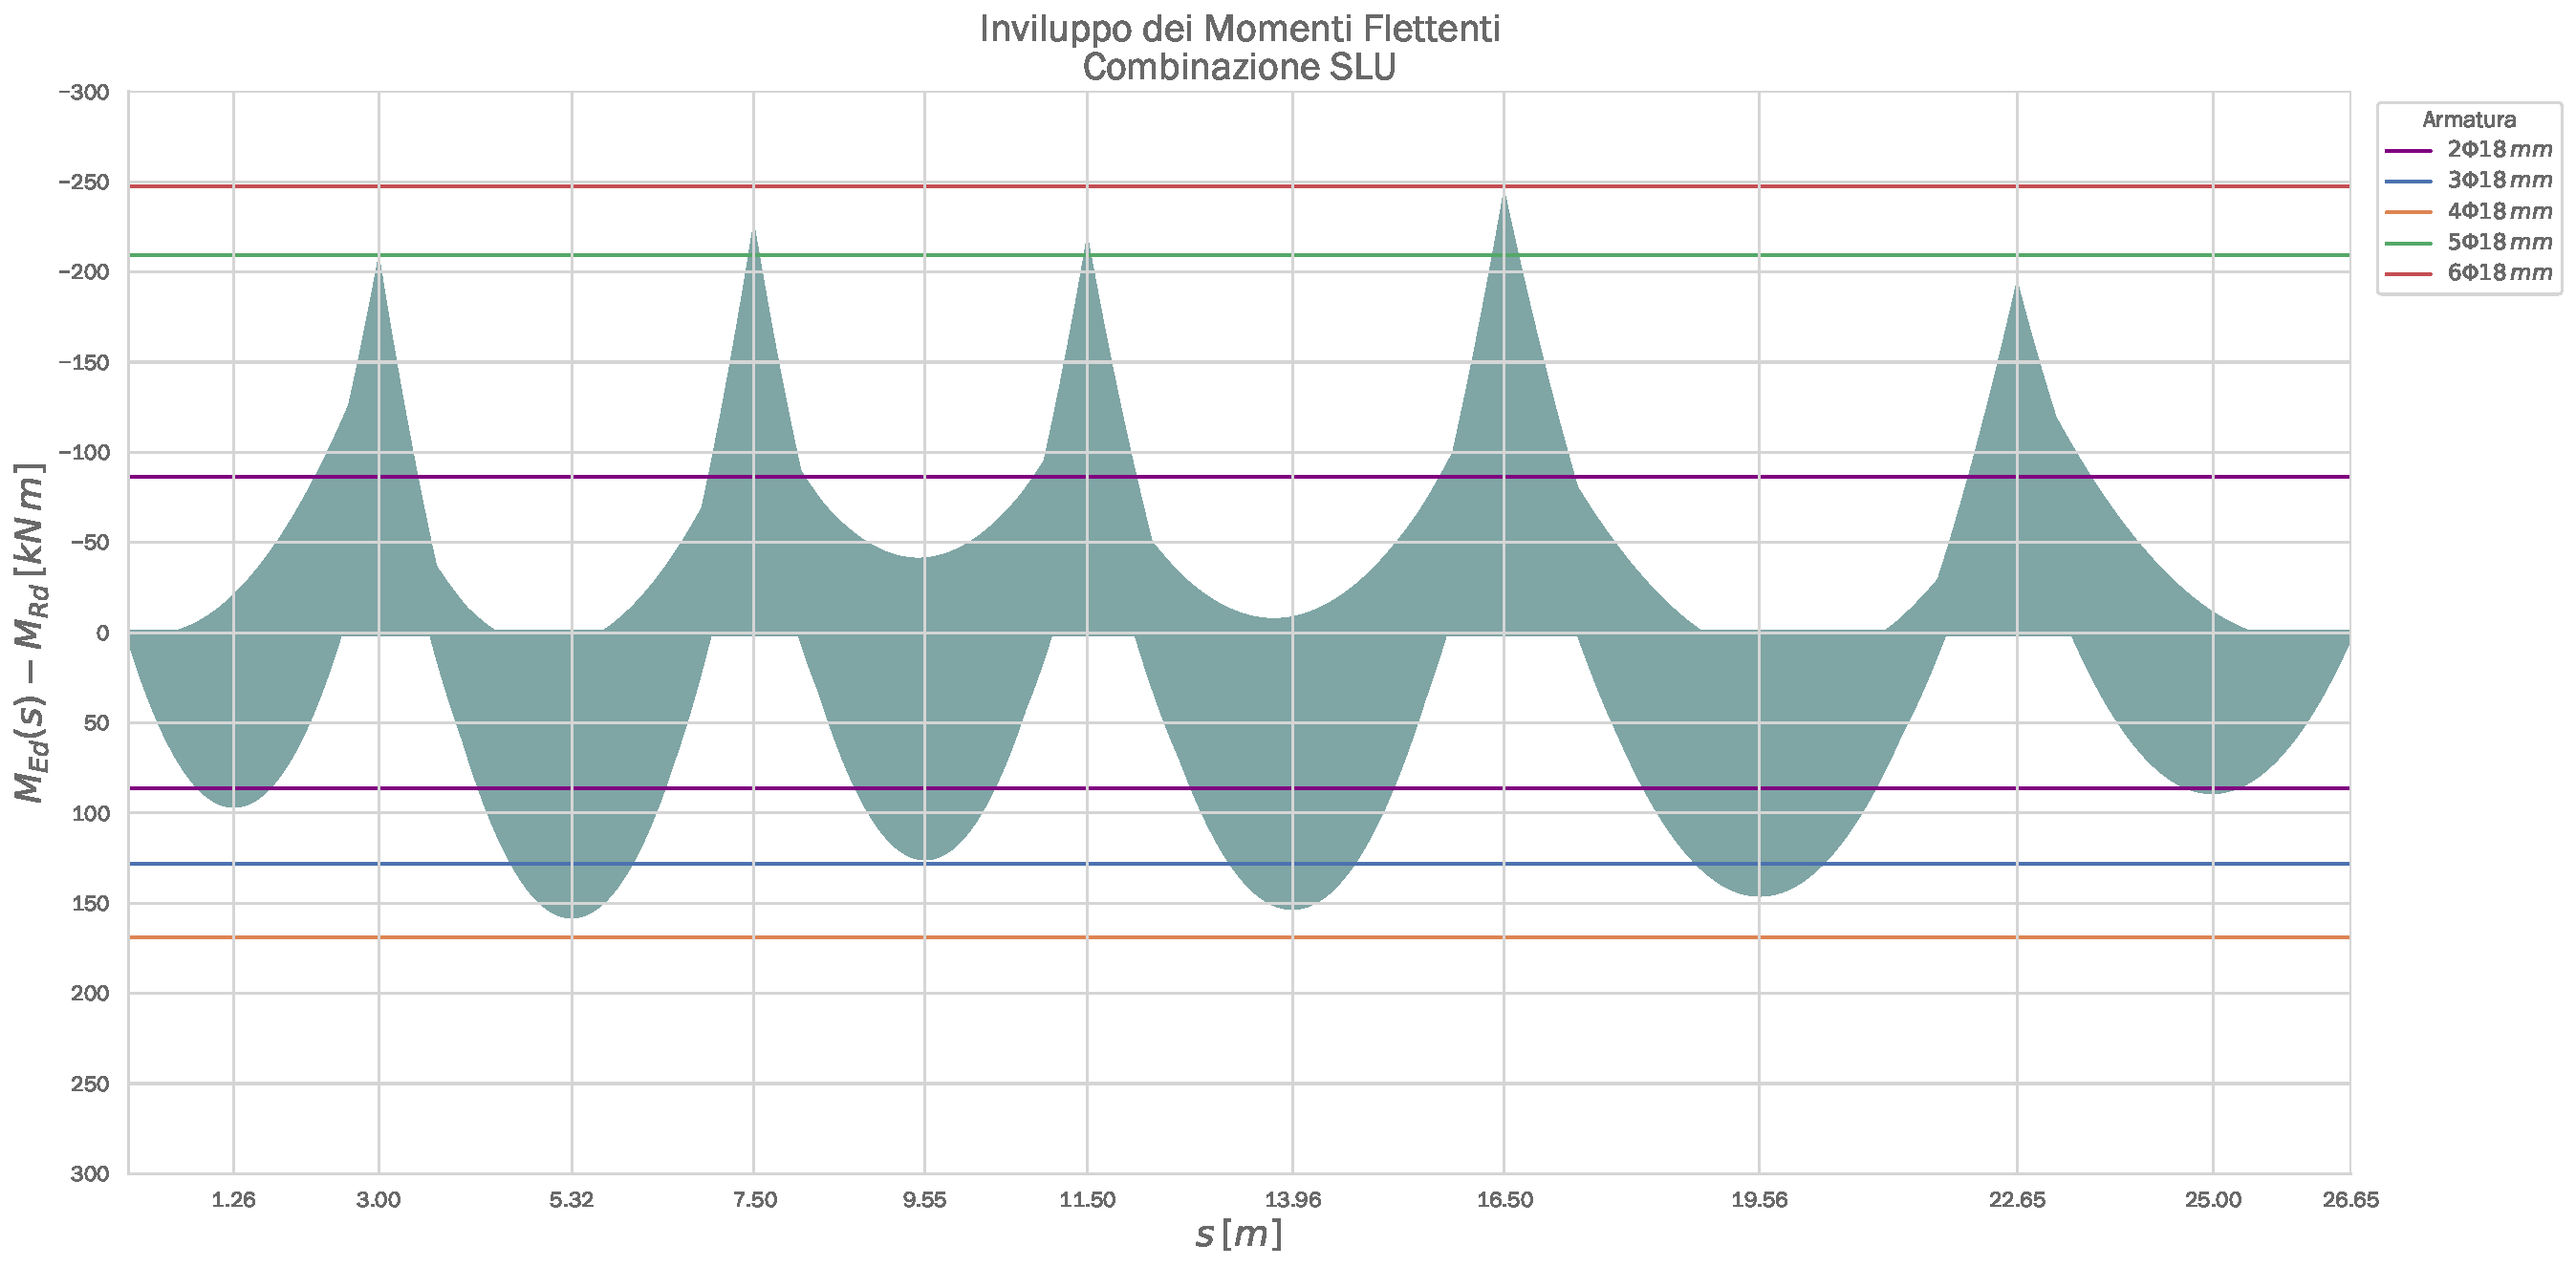
\includegraphics[width=\textwidth]{MEd-MRd_beam_slu}
	\caption{Sovrapposizione momenti sollecitanti e momenti resistenti}
	\label{fig:MEd-MRd}
\end{figure}

I valori principali sono riassunti nelle tabelle~\ref{tab:verificaSezione_slu} e \ref{tab:verificaSezioneInvertita_slu}. Inoltre, in figura~\ref{fig:MEd-MRd} è rappresentata la Sovrapposizione dei momenti flettenti sollecitanti e dei momenti resistenti della sezione, in funzione dell'armatura.

\section{Verifica sulle armature}
\`E ora necessario fare un controllo geometrico sulla sezione, oltre ai controlli richiesti dalla normativa; si deve, infatti, accertare se il numero di barre d'armatura scelto sta effettivamente nella base $b = 300\,mm$. In particolare, l'\textbf{EC2} riporta la seguente relazione per la spaziatura fra le barre
\[
s_{min} = \max\left\{k_1\,\Phi_l; d_g + k_2; 20\,mm\right\}
\]
dove, dal \textbf{NAD} $k_1 = 1$ e $k_2 = 5\,mm$. Perciò
\[
s_{min} = \max\left\{18\,mm; 25\,mm ; 20\,mm\right\} = 25\,mm
\]

Considerando un diametro delle staffe $\Phi_{st} = 8\,mm$ e un copriferro laterale di $c = 20\,mm$, la base minima per contenere $6\,\Phi\,18\,mm$ è di

\begin{align*}
	b_{min} &= 2\,c + n_b\,\Phi_{st} + n\,\Phi_l + (n-1)\,s_{min} = 2\cdot 20\,mm + 2\cdot 8\,mm + 6\cdot 18\,mm + 5\cdot 25\,mm =\\
	&=289\,mm < b = 300\,mm
\end{align*}
dove $n_b$ è il numero di bracci delle staffe ($n_b = 2$) e $n$ è il numero di barre longitudinali.

Le \ntc impongono una verifica sul quantitativo di armatura: in zona tesa si deve avere un minimo di 

\[
A_{s,min} = \dfrac{0.26\,f_{ctm}}{f_{yk}}\,b_t\,d = \dfrac{0.26\cdot 2.57}{391.30}\cdot 300\cdot 460 = 235.66\,mm^2 > 0.0013\,b_t\,d = 179.40\,mm^2
\]

L'armatura minima in zona tesa è di $3\,\Phi\,18$, cioè 
\[
A_s = 3\,\Phi\,18 = 763.41\,mm^2 > A_{s,min}
\]

Vi è un vincolo anche sul quantitativo massimo di armatura che deve essere inferiore di 
\[
A_{s,max} = 0.04\,A_c = 0.04\cdot 300\cdot 500 = 6000\,mm^2
\]

L'armatura massima (in trazione o compressione) è di
\[
A_s = 6\,\Phi\,18 = 1526.81\,mm^2 < A_{s,max}
\]

Infine la normativa impone un minimo di due barre in ogni zona (tesa e compressa) e almeno una barra per spigolo. 


\section{Traslazione del diagramma dei momenti flettenti}\label{sec:traslazioneMomenti}
Per via dell'azione assiale di trazione generata dal taglio sulle armature tese quest'ultime saranno sollecitate da uno sforzo assiale maggiore di quello calcolato per la sola azione del momento flettente descritto in precedenza. Per questo motivo è necessario tener conto del contributo dell'azione tagliante, che però risulta essere variabile lungo l'asse della trave. La normativa italiana viene incontro a questo problema nel punto \textbf{4.1.2.3.5.2}, dove definisce la formula di traslazione del diagramma dei momenti flettenti sollecitanti. In particolare, la \textit{$[4.1.30]$} riporta
\[
    a_1 = (0.9\cdot d\cdot \cot\theta)/2
\]
dove $0.9\cdot d$ è il braccio di leva delle forze interne e $\theta$ è l'inclinazione dei puntoni compressi in calcestruzzo rispetto all'asse longitudinale della trave. L'angolo $\theta$ è limitato inferiormente e superiormente dalla normativa, che impone il seguente intervallo
\[
    1\leq \cot\theta\leq 2.5
\]

A favore di sicurezza, si sceglie il valore riferito al limite superiore: $\cot\theta = 2.5$; da cui
\[
    a_1 = (0.9\cdot 460\,mm\cdot 2.5)/2 = 517.5\,mm\simeq 518\,mm
\]

\begin{figure}
    \centering
	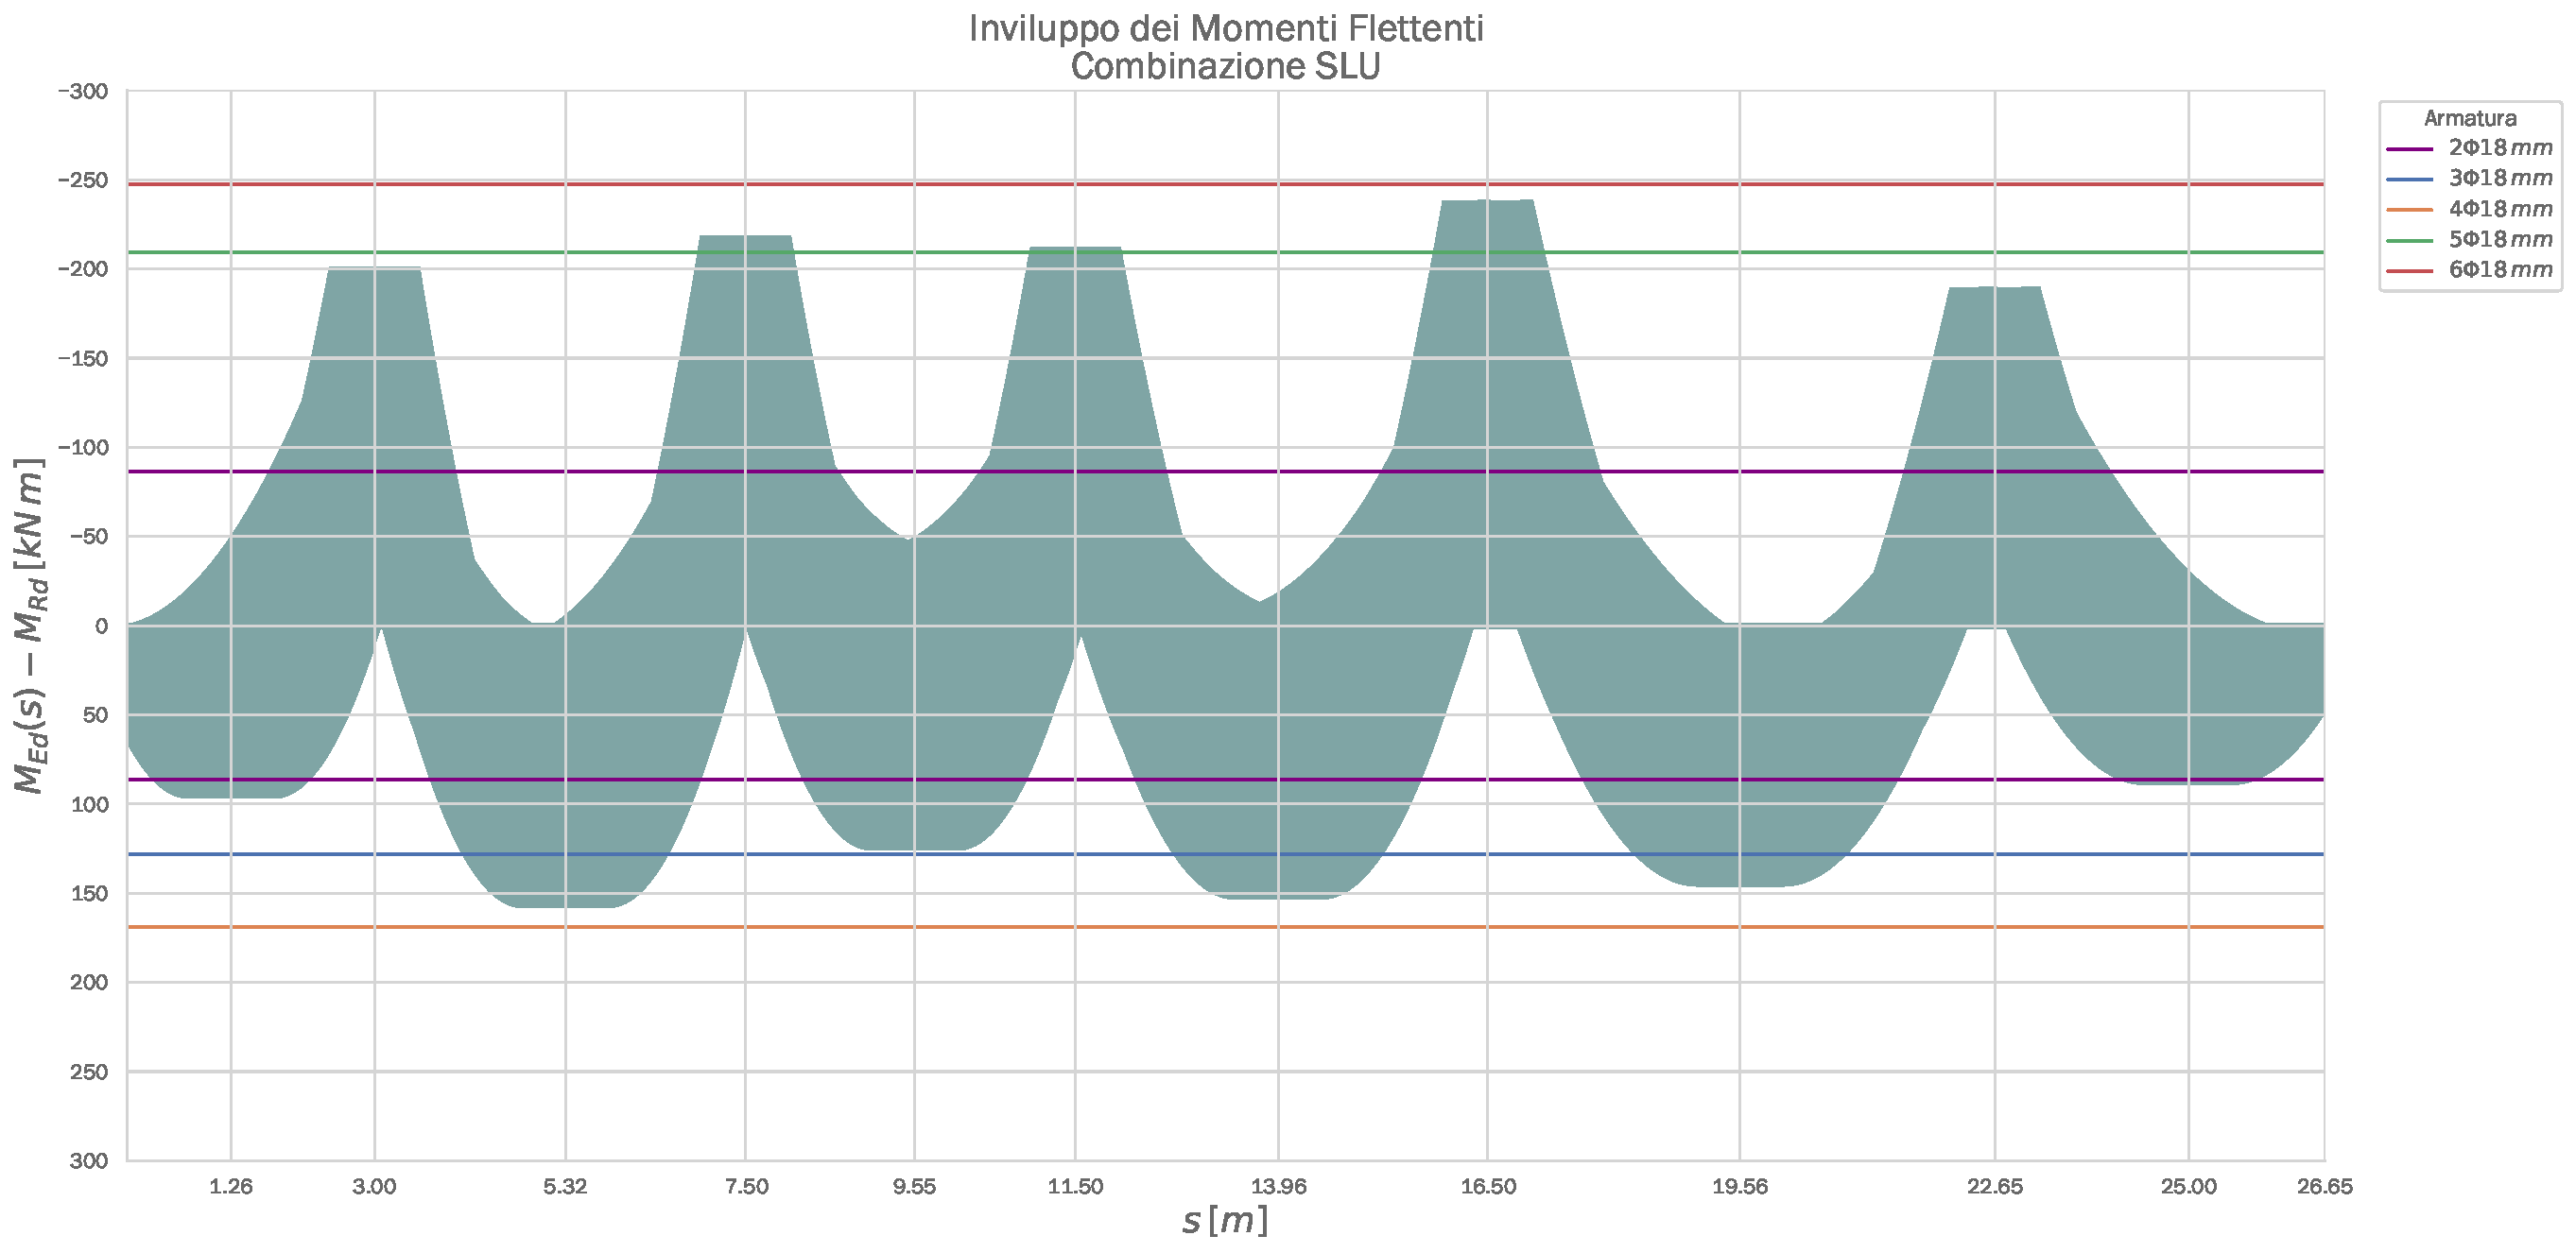
\includegraphics[width=\textwidth]{MEd-MRd_traslato_beam_slu}
	\caption{Sovrapposizione diagramma dei momenti sollecitanti traslato e momenti resistenti}
	\label{fig:MEd-MRd_traslato}
\end{figure}

Il diagramma traslato è rappresentato in figura~\ref{fig:MEd-MRd_traslato}.

\begin{figure}
	\centering
	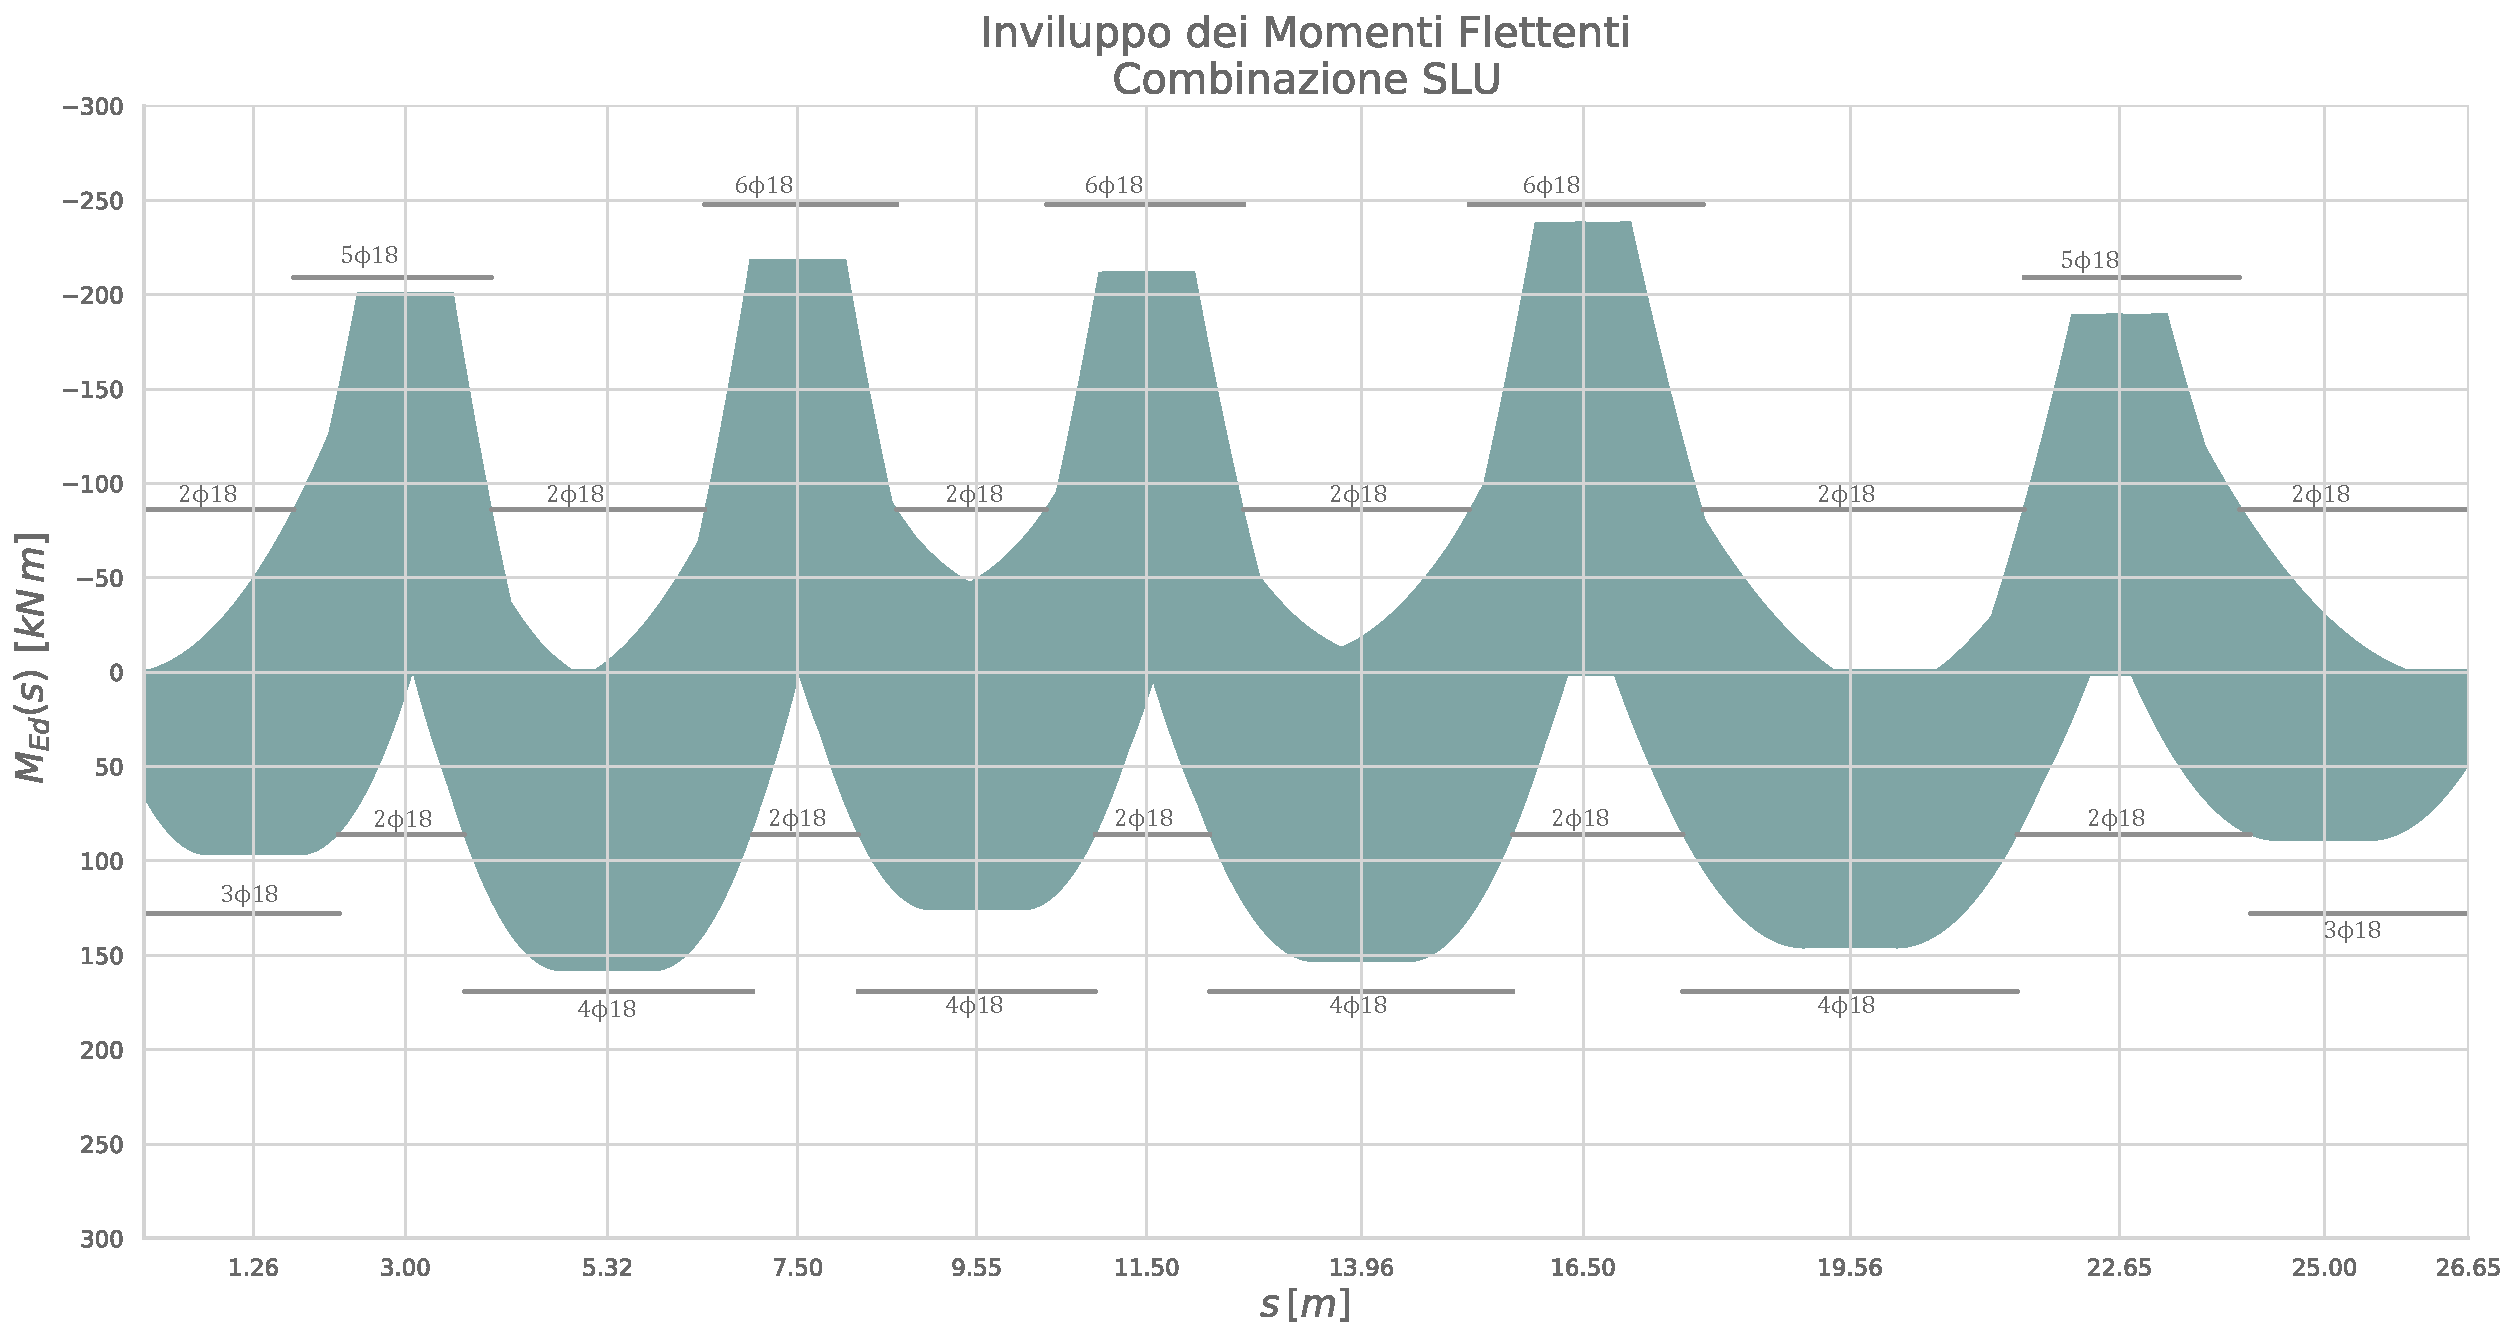
\includegraphics[width=\textwidth]{MEd-MRd_armature}
	\caption{Disposizione delle armature} 
	\label{fig:MEd-MRd_armature}
\end{figure}

Dalla Sovrapposizione dei momenti resistenti al diagramma dei momenti sollecitanti si può disegnare una prima approssimazione della disposizione delle armature, che risulta essere come in figura~\ref{fig:MEd-MRd_armature}. Partendo da questo, si dovranno calcolare le lunghezze di ancoraggio delle barre che andranno a sovrapporsi le une alle altre.

\section{Lunghezze di ancoraggio}\label{sec:ancoraggio}
Affinché l'armatura possa lavorare al meglio delle sue prestazioni meccaniche necessita di valutare la lunghezza di ancoraggio delle barre (principalmente tese, ma anche compresse). Idealmente lungo questa lunghezza la tensione nell'armatura deve passare da un valore nullo all'estremità della barra, al valore di tensione di lavoro considerata durante il progetto. Avendo ipotizzato, nel progetto, l'armatura tesa in condizioni di collasso, si sceglie un valore di tensione di lavoro pari alla tensione di snervamento di progetto $f_{yd}$. Si suppone, inoltre, che la tensione di ancoraggio vari linearmente con la lunghezza. 

L'\textbf{EC2}, nel punto \textbf{8.4.4} descrive il procedimento per il calcolo delle lunghezze di ancoraggio:
\[
l_{bd} = \alpha_1\,\alpha_2\,\alpha_3\,\alpha_4\,\alpha_5\,l_{b,rqd} \geq l_{b,min}
\]
dove $\alpha_1$ dipende dalla forma della barra ancorata, $\alpha_2$ tiene conto del copriferro, $\alpha_3$ considera l'effetto di confinamento delle staffe, $\alpha_4$ tiene conto di eventuali barre saldate e infine $\alpha_5$ tiene in considerazione la pressione trasversale che riduce - anche se di poco - la lunghezza di ancoraggio finale. La lunghezza di ancoraffio richiesta $l_{b,rqd}$ è definita dalla formula $(8.3)$ dell'eurocodice 2:
\[
l_{b,rqd} = \dfrac{\Phi}{4}\,\dfrac{\sigma_{sd}}{f_{bd}}
\]
che dipende, come si può vedere, dal diametro delle barre. La tensione $\sigma_{sd}$ è la tensione di progetto in cui le barre lavorano alla lunghezza di ancoraggio e, come detto sopra, viene scelta pari a $f_{yd}$. Il termine $f_{bd}$ è la tensione massima di aderenza del calcestruzzo e si calcola come
\[
f_{bd} = 2.25\,\eta_1\,\eta_2\,f_{ctd}
\]

Si ipotizza una condizione di \textit{buona aderenza} e perciò $\eta_1 = 1$, mentre impiegando solamente barre d'armatura di diametro $\Phi\,18 < \Phi\,32$, anche il coefficiente $\eta_2$ risulta unitario. Il valore della tensione a trazione di progetto del calcestruzzo è stato calcolato alla \eqref{eq:fctd} (a pagina~\pageref{eq:fctd}) e vale $f_{ctd} = 1.02\,MPa$. Allora
\[
f_{bd} = 2.25\cdot 1\cdot 1\cdot 1.02\,MPa = 2.295\,MPa \simeq 2.30\,MPa
\]

Sostituendo 
\[
l_{b,rqd} = \dfrac{18\,mm}{4}\,\dfrac{391.30\,MPa}{2.30\,MPa} = 765.59\,mm \simeq 766\,mm
\]

Il valore minimo di lunghezza di ancoraggio è di 
\begin{align*}
	l_{b,min} \geq \begin{cases}
		\max\{0.3\,l_{b,rqd}; 10\,\Phi; 100\,mm\} &= \max\{229.80\,mm; 180\,mm; 100\,mm\} =\\ &= 229.80\,mm\simeq 230\,mm \quad \text{per armature tese}\\
		\max\{0.6\,l_{b,rqd}; 10\,\Phi; 100\,mm\} &= \max\{459.60\,mm; 180\,mm; 100\,mm\} =\\&= 459.60\,mm\simeq 460\,mm \quad \text{per armature compresse}
	            \end{cases}
\end{align*}

\begin{figure}
	\centering
	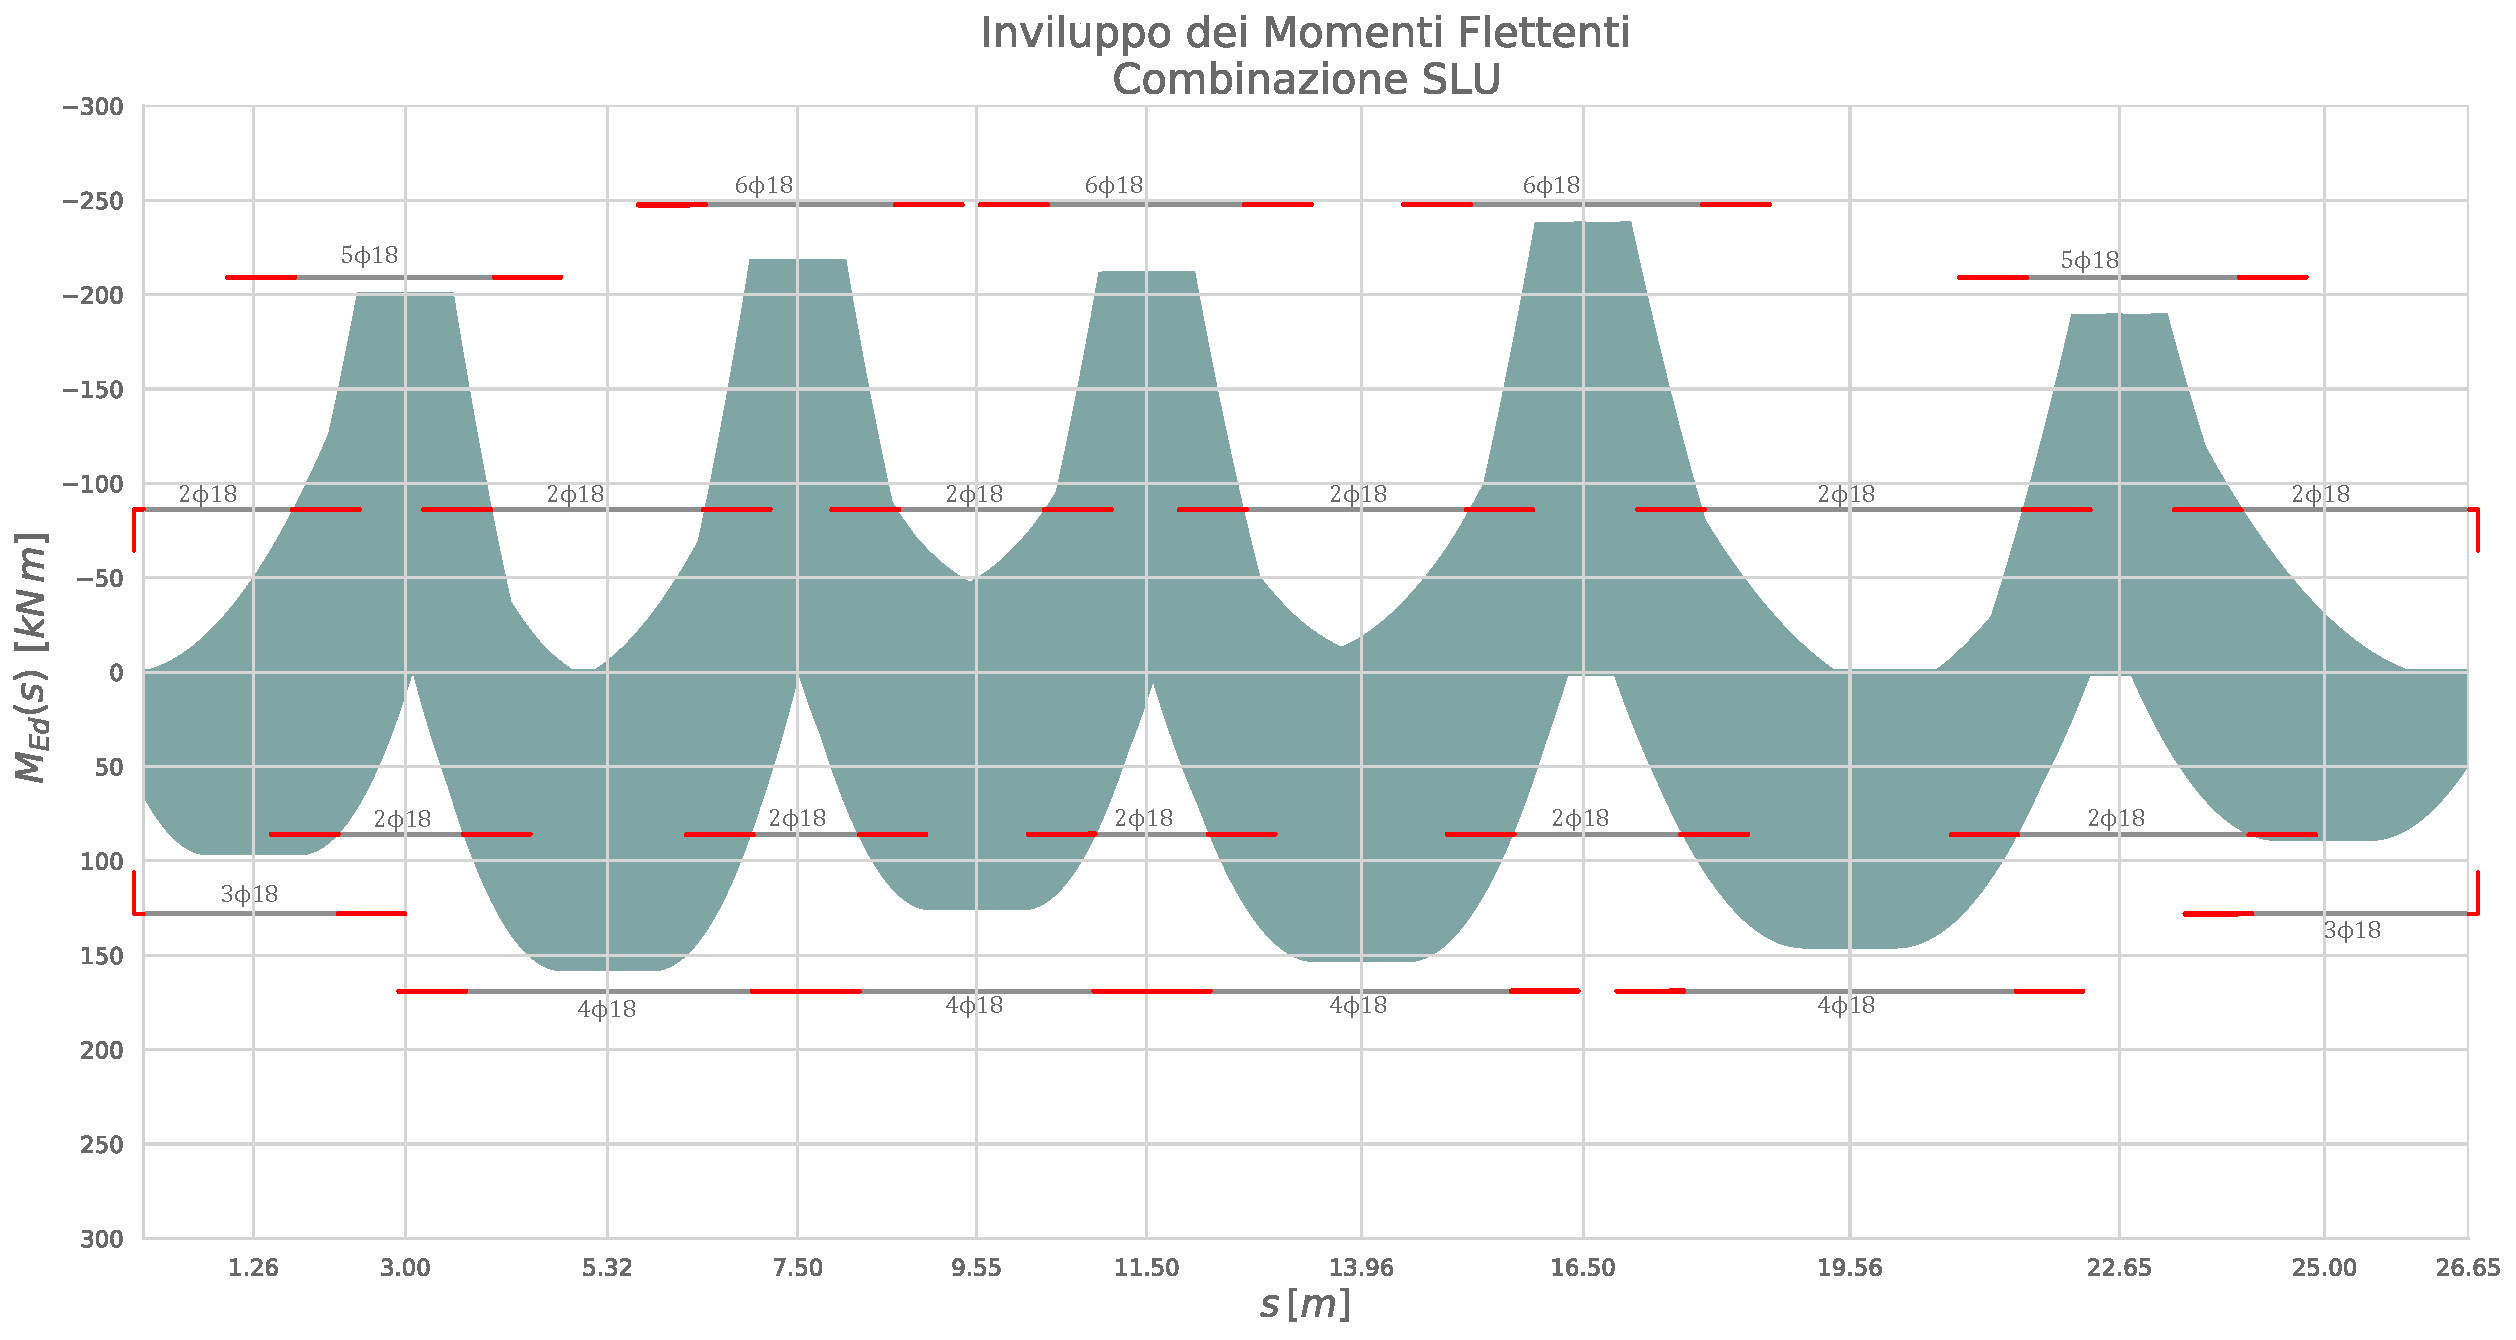
\includegraphics[width=\textwidth]{MEd-MRd_ancoraggio}
	\caption{Disposizione delle armature e ancoraggio delle barre} 
	\label{fig:MEd-MRd_ancoraggio}
\end{figure}

Poiché si considerano ancoraggi con barre rettilinee $\alpha_1 = 1$; mentre, non essendoci barre saldate. $\alpha_3 = \alpha_4 = 1$  Infine, sempre a favore di sicurezza si assume la pressione trasversale sulle barre nulla, da cui $\alpha_5 = 1$. Per il calcolo di $\alpha_2$, si considera la spaziatura $a$, calcolata come
\[
a = \dfrac{b - 2\,c - n_b\,\Phi_{st}-n\,\Phi_l}{n-1} = 26.40\,mm
\]

Allora
\[ 
c_d = \min\left\{\dfrac{a}{2}; c_1; c\right\} = 13.20\,mm
\]
e
\[
\alpha_2 = 1-0.15\,\dfrac{c_d - \Phi_l}{\Phi_l} = 1.04 \nless 1 ~ \Longrightarrow~ \alpha_2 = 1
\]


La lunghezza di ancoraggio vale, perciò
\[
l_{bd} = 1\cdot1\cdot1\cdot1\cdot1\cdot 766\,mm = 766\,mm\simeq 770\,mm > \begin{cases}
	230\,mm \quad \text{in tensione}\\
	460\,mm \quad \text{in compressione}
                                                                  \end{cases}
\]

% \begin{figure}
% 	\centering
% 	\includegraphics[height=\textwidth, angle=90]{../../disposizioneArmature}
% 	\caption{Disposizione delle armature nella trave} 
% 	\label{fig:disposizioneArmature}
% \end{figure}
\pagebreak
\thispagestyle{empty}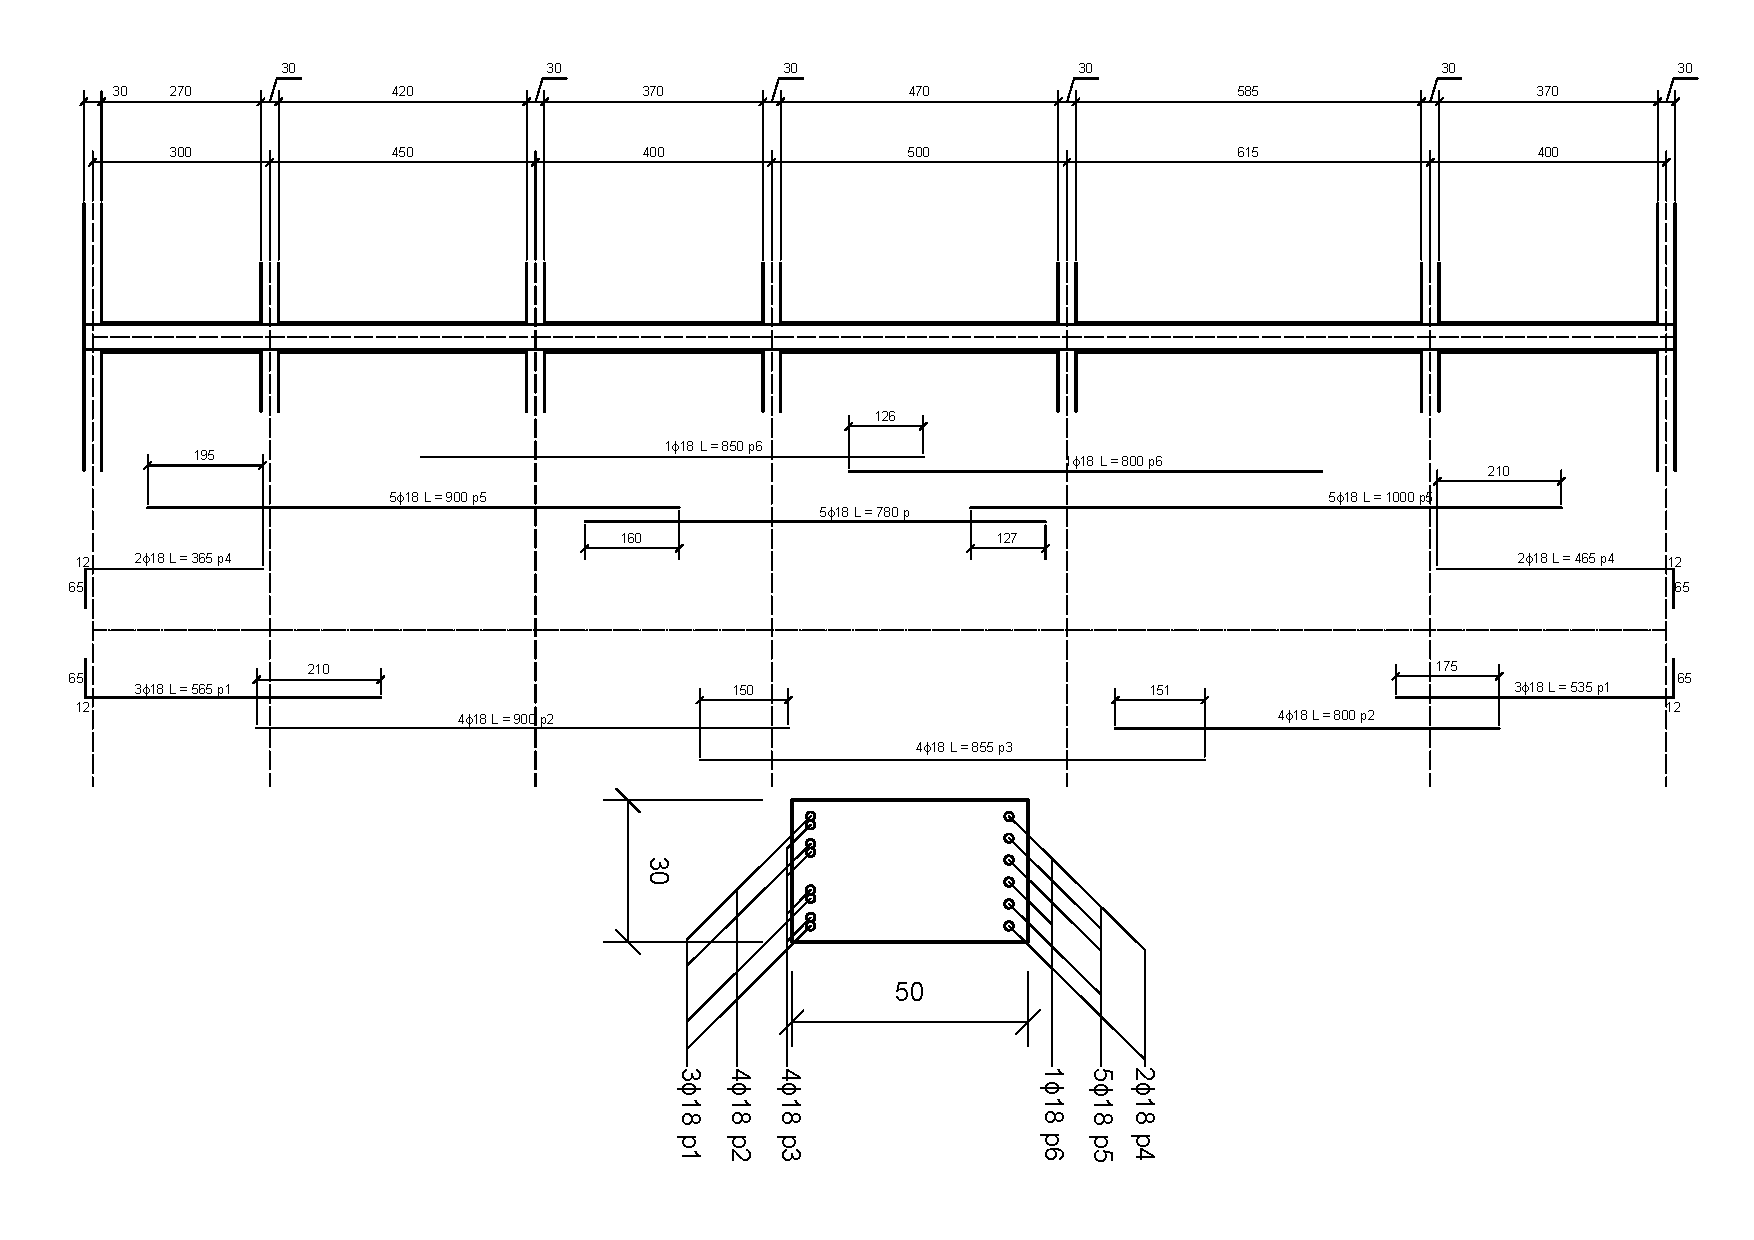
\includepdf[pages=1,pagecommand={}, angle=90, width=\textwidth]{../../disposizioneArmatureFlessione}
\cleardoublepage
